\section{Introduction}
Today, mass surveillance and censorship severely threaten democracy and freedom of speech. Governments around the world control the Internet to protect their domestic political, social, financial, and security interests. This makes anonymity a crucial tool for preserving privacy of individuals in cyberspace. Tor~\cite{dingledine:2004} is the most popular anonymous communication network with more than 2.5 million users per day~\cite{Tor:Users}. Tor relays the Internet traffic via more than 6,000 volunteer nodes called \emph{relays} spread across the world. Tor users can connect to the network and have their Internet data routed through the network before reaching any server, thus the servers are not able to distinguish between Tor users or locate them. 

Since the list of all relays is available publicly, state-sponsored organizations can enforce Internet service providers (ISPs) to block access to all of them making Tor unavailable in territories ruled by the state. When access to the Tor network is blocked, Tor users have the option to use \emph{bridges} -- volunteer relay nodes that are not all listed in Tor's public directory~\cite{Dingledine06designof}. Bridges serve only as entry points into the rest of the Tor network, and their addresses are carefully distributed to the users, with the hope that they cannot be all learned by censorship authorities. Tor users behind censorship firewalls must find bridges through email, uncensored web sites, etc.

Although currently the bridges are distributed among the users based on different strategies such as CAPTCHA-enabled email-based distribution and IP-based distribution~\cite{Dingledine06designof}, studies indicate that censors are using sophisticated mechanisms along with a large coalition of corrupt users (scanners) to obtain and block many bridge addresses rendering Tor unavailable for many users~\cite{Dingledine:Bridges:2011,BridgeBlockingChina:2012,Ensafi2015b}.

In this paper, we study the problem of bridge distribution in Tor, where a set of bridges is distributed among $n$ users, $t$ of whom are controlled by a censor, in such a way that all honest users can access a bridge that is not blocked by the censor. A solution to this problem would allow us to make the Tor network provably available for all users.
Unfortunately, state of the art techniques for bridge distribution either cannot guarantee that all honest users can access Tor~\cite{WangLBH:rBridge:13,McCoy:FC:2011} or only work when $t$ is known in advance~\cite{Mahdian:2010}. 

In contrast, we describe an algorithm that ensures Tor is available to all honest users with high probability without requiring any \emph{a priori} knowledge about $t$. 
It is often hard in practice to estimate the number of corrupt users due to the sophisticated nature of Internet censorship in many countries such as China~\cite{Oni:2012:China,Ensafi2015b}. Moreover, censors can easily implement strategies to prevent the circumvention mechanism from correctly estimating the number of corrupt users.

Inspired by the \emph{resource competitive analysis} approach of Gilbert~\etal~\cite{Gilbert:2012:RAN:2335470.2335471} and Bender~\etal~\cite{Bender:2015:SIGACT}, our algorithms provide the following guarantee: if the adversary pays $t$ amount of resource cost, then the resource cost of our algorithms is some function of $t$. This allows us to achieve near-optimal resource costs with strong robustness to disruptions caused by the censor.

Our main strategy for preventing the censor from blocking a large fraction of the bridges is to use randomization. This is because the colluding censor cannot predict the behavior of the randomized process in distributing a set of bridges to the users, and thus it cannot arrange its corrupt users in such a way that prevents some of the honest users from connecting to the Tor network. Moreover, our algorithm can adaptively adjust the number of bridges required based on the number of bridges compromised so far and guarantees that the number of rounds until all honest users can connect to Tor is bounded by $O(\log{t})$. Our algorithms can be run independently from Tor; the Tor network remains intact to focus on its main purpose of providing anonymity.

In Section~\ref{sec:model}, we describe our communication and adversarial model. In Section~\ref{sec:results}, we state our main theorem. We review the previous results and related work in Section~\ref{sec:relatedwork}. In Section~\ref{sec:algorithm}, we describe our algorithms for reliable bridge distribution; we start from a simple algorithm and improve it as we continue. We summarize the paper and state a few open problem in Section~\ref{sec:conclusion}.

\subsection{Our Model} \label{sec:model}
Consider $n$ users connected to the Internet via an ISP inside a censorship territory. We consider two distribution models: \emph{single-distributor} and \emph{multi-distributor}. In the former model, we assume a single trusted server called the \emph{bridge distributor} (or simply the \emph{distributor}) connected to the Internet via an ISP outside the territory. The distributor has information about a set of $m$ Tor bridges that are also located outside the territory. Each user is willing to obtain a list of bridge addresses at least one of which can be used to connect to Tor network. The user sends its request for bridges to the distributor using a rate-limited channel\footnote{A vital communication mechanism such as Gmail that the censor cannot block due to major economic and political consequences, but is not suitable for interactive communication over the Internet such as web surfing.} such as email, and the distributor runs one of our algorithms to send a set of bridge addresses back to the user via the same channel.

We consider an adversary (the \emph{censor}) who controls $t$ of the users and is \emph{adaptive} 	 meaning that it can choose the set of \emph{corrupt users} at the beginning of each round of communication, but is limited to corrupting at most $t$ users combined in all rounds. We refer to the other ${n-t}$ users as \emph{honest users}.
The adversary is willing to learn as many bridges addresses as possible via its set of corrupt users in order to block the bridges. However, it does not have to block a bridge as soon as it finds the address; it is allowed to strategically (perhaps by colluding with other corrupt users) decide when to block a bridge. We assume our algorithms do not have any knowledge about the number of corrupt users, $t$, before they begin, and the adversary has no knowledge about the randomness generated by the distributor throughout the algorithms other than what it can learn from the bridges assigned to the corrupt users.

In the multi-distributor model, a set of $d$ distributors collaborate with each other to distribute bridge addresses among the users such that none of the distributors can learn any information about the bridge addresses and/or the bridge-user assignments. In this model, the adversary not only can corrupt an unknown number of the users, $t$, but also can maliciously control and read the internal state of up to $\lceil d/3 \rceil$ of the distributors. The corrupt distributors can deviate from our protocols in any arbitrary manner, \eg, by sending invalid messages or remaining silent. Figure~\ref{fig:model} depicts our model. In all of our figures, we mark adversary-controlled nodes with a horn.

\begin{figure*}[t]
	\centering
	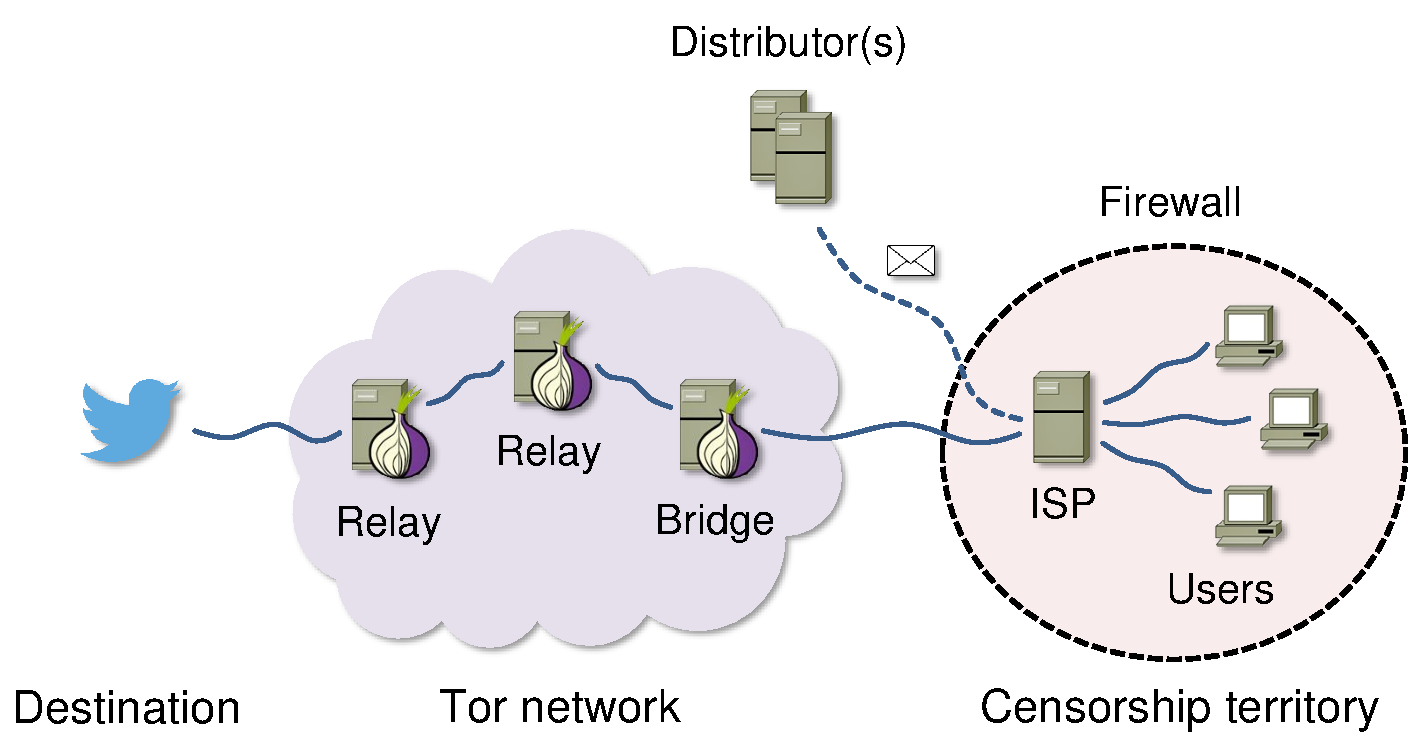
\includegraphics[width=0.62\linewidth]{images/model}
	\caption{Our model}
	\label{fig:model}
\end{figure*}

\subsection{Our Results} \label{sec:results}
\noindent We prove the following main theorem in Section~\ref{sec:ProofSimple}.
\begin{theorem}
	\label{thm:main} There exists bridge distribution protocols that guarantee the following properties with probability ${1 - 1/n^k}$, for some constant ${k \geq 1}$: % change this to ``at least with probability 1-1/n^c'' %
	\begin{enumerate}
		\item All honest users can connect to Tor after ${\lceil \log{t} \rceil + 2}$ rounds of communication with the distributor(s);
		\item The total number of bridges required is $O(t\log{n})$;
		\item Each user sends/receives $O(\log{n})$ bits in the single-distributor model and $O(d\log{n})$ bits in the multi-distributor model.
	\end{enumerate}
\end{theorem}

The best known algorithm for bridge distribution~\cite{Mahdian:2010} only works when the number of corrupt users, $t$, is known in advance and requires at most ${t\left(1 + \lceil \log{(n/t)} \rceil \right)}$ bridges. In contrast, our algorithms not only do not require any prior knowledge about $t$ but also use fewer bridges.\todo{What?? $O(t\log{n})$ isn't fewer than~\cite{Mahdian:2010}}

\section{Related Work} \label{sec:relatedwork}
%The development of Tor started as a research project in 1995 at the US Naval Research Laboratory. The Tor Network became operational in 2003 and since 2006 it has been maintained and improved by Tor Project Inc., a US non-profit organization.
The bridge distribution problem can be seen as a special case of the proxy distribution problem, where a set of unblocked servers (proxies) outside the censorship territory are distributed among the users inside the territory. These proxies are used to relay Internet traffic to blocked websites. The proxy distribution problem has been studied by several previous work. 

Feamster~\etal~\cite{Feamster:PETS:2003} propose a proxy distribution algorithm that requires every user to solve a cryptographic puzzle to discover a proxy. This way, the algorithm prevents the corrupt users from learning a large number of proxies. Unfortunately, empirical results of~\cite{Feamster:PETS:2003} show that a computationally powerful censor can easily block a very large fraction of the proxies.

The Kaleidoscope system of Sovran~\etal~\cite{Sovran:2008:PSN} disseminates proxy addresses over a social network whose links correspond to existing real world social relationships among users. Unfortunately, this algorithm assumes the existence of a few internal trusted users who can relay other users' traffic and cannot guarantee its users' access to Tor.

McCoy~\etal~\cite{McCoy:FC:2011} propose Proximax; a proxy distribution system that uses social networks such as Facebook as trust networks that can provide a degree of protection against discovery by censors. Proximax estimates each user's effectiveness and chooses the most effective users for advertising proxies with the goals of maximizing the usage of these proxies while minimizing the risk of having them blocked.

Even if bridges are distributed carefully among the users, censors can still block access to the Tor network via deep packet inspection (DPI). The Tor Project has developed a variety of tools under the name \emph{pluggable transports}~\cite{Tor:PluggableTransport} that can be used to obfuscate the traffic transmitted between the client and the bridge. This makes it hard for the censor (who monitors the traffic) to distinguish between the legitimate-looking obfuscated traffic and the actual Tor traffic. Although pluggable transports are necessary for preventing bridge blocking via DPI, they cannot prevent blocking via colluding corrupt users. Moreover, recently Wang~\etal~\cite{Wang:2010:CCS} showed that current obfuscation mechanisms used in Tor can be reliably detected by censors with sufficiently low false-positive rates. In our model, we assume our algorithm runs in parallel with a reliable pluggable transport tool that can prevent DPI blocking.

Mahdian~\cite{Mahdian:2010} studies the proxy distribution problem when the number of corrupt users, $t$, is known in advance. He proposes algorithms for both large and small values of $t$ and provides a lower bound for dynamic proxy distribution that is useful only when ${t \ll n}$.\footnote{ For large values of $t$ (\eg, ${t = cn}$ for ${c \in (0,1)}$) the trivial lower bound of $\Omega(t)$ is better than ${\Omega\left(\frac{t\log{(n/t)}}{\log{t} +\log{\log{n}}}\right)}$ of~\cite{Mahdian:2010}.} Unfortunately, it is usually hard in practice to reliably estimate the value of $t$. Mahdian's algorithm for large known $t$ requires at most ${k\left(1 + \lceil \log{(n/k)} \rceil \right)}$ bridges, and his algorithm for small known $t$ uses ${O(k^2 \log{n} / \log{\log{n}})}$ bridges.

Wang~\etal~\cite{WangLBH:rBridge:13} propose a reputation-based bridge distribution mechanism called rBridge that computes every user's reputation based on the uptime of its assigned bridges and allows the user to replace a blocked bridge by paying some reputation credits. Interestingly, rBridge is the first model to provide user privacy against an honest-but-curious distributor. This is achieved by performing oblivious transfer between the distributor and the users along with commitments and zero-knowledge proofs for achieving unlinkability of transactions.

Our algorithms rely on a technique for testing reachability of bridges from outside the censored territory. Dingledine~\cite{Dingledine:BridgeReach:2011} and Ensafi~\etal~\cite{Ensafi:2014:PAM} describe active scanning mechanisms for testing availability of bridges. The details of these methods and their current challenges are out of scope of our paper.

%In a line of research, Winter and Lindskog~\cite{BridgeBlockingChina:2012}, Winter and Crandall~\cite{Winter:2012:login}, and Ensafi~\etal~\cite{Ensafi2015b} examined China's \emph{active probing} mechanisms against current enhanced circumvention mechanisms of Tor. By recruiting nodes that act like users, the censor passively monitors the network for suspicious traffic, actively probes the corresponding servers, and blocks those determined to run Tor.

%\section{Preliminaries} \label{sec:preliminaries}
%We now define our notation and describe the tools used throughout this paper.
	
\section{Our Algorithms} \label{sec:algorithm}
\todo{update this paragraph before submission.} In this section, we first construct a bridge distribution algorithm that adaptively increases the number of bridges used with respect to the number of bridges blocked. In Section~\ref{sec:ProofSimple}, we prove the desired properties of this algorithm. In Section~\ref{sec:Fixed}, we improve our result by constructing a detection-and-eviction mechanism, where blocking parties are gradually detected and removed from the algorithm. We show properties of this algorithm in Section~\ref{sec:ProofFixed}.
Before proceeding to our algorithms, we define the standard terms and notation used throughout our paper. 
\begin{description}
	\item[Notation.] We say an event occurs \emph{with high probability}, if it occurs with probability at least \emph{${1-1/n^k}$}, for some constant ${k \geq 1}$. We denote the set of integers ${\{1,...,n\}}$ by $[n]$. We denote a set of $n$ users participating in our algorithms by ${\{u_1,...,u_n\}}$. We say a bridge is \emph{blocked} when the censor has restricted users' access to this bridge. We refer to the remaining bridges as \emph{unblocked} bridges.
\end{description}

\subsection{Single-Distributor Algorithm}
Our basic method is a Monte Carlo algorithm that proceeds in rounds (see \mbox{Algorithm~\ref{alg:MainSimple}}): In each round, the algorithm randomly distributes a set of bridges among the users and proceeds to the next round once the number of blocked bridges exceeds a threshold that is increased exponentially in each round. In every round, the number of bridges distributed is increased with respect to the number of bridges blocked so far. In any round, if the number of bridges to be distributed is larger than the number of users, $n$, then the algorithm assigns a unique bridge to every user.

\begin{algorithm}[t]
	\caption{High-Level Bridge Distribution Scheme}
	\label{alg:MainSimpleShort}
	
	\algFont \vspace{2pt}
	\begin{algorithmic}[1]
		\State Initialize parameters: ${i \gets 0}$; ${b_i \gets 1}$
		\While{\True}
			\If {$b_i \geq 2^i$} \label{ln:ConditionSimple}
				\State $i \gets i+1$ \label{ln:IncrementSimple}
				\State Distribute $2^i$ bridges: \label{ln:DistributeSimple}
				\Indent
					\therule \ForAll{users}
						\State Pick a bridge randomly
						\State Assign the user to the bridge
					\EndFor
				\EndIndent
			\EndIf
			\State $b_i \gets$ \# bridges blocked
		\EndWhile
	\end{algorithmic}
\end{algorithm}

%We later show that each run of Algorithm~\ref{alg:MainSimple} guarantees that all users can connect to Tor with some constant probability. Thus, if the distributor repeats the algorithm ${O(\log{n})}$ times in parallel, it can guarantee that all users can connect to Tor with high probability.

\begin{algorithm}[t]
	\caption{Bridge Distribution Scheme}
	\label{alg:MainSimple}
	
	\algFont \vspace{2pt}
	\begin{algorithmic}[1]
		\State Initialize parameters: ${nextRound \gets \True}$; ${i \gets 0}$; $U \gets$ a set of users ${\{u_1,...,u_n\}}$
		\While{\True}
			\If {$nextRound$} \label{ln:ConditionSimple}
				\State $i \gets i+1$ \label{ln:IncrementSimple}
				\If {$2^ic\log{n} < n$}
					\ForAll{$j \in [c\log{n}]$}
						\State $B_{ij} \gets$ a list of $2^i$ bridges
						\State \Call{Distribute}{$U, B_{ij}$} \label{ln:DistributeSimple}
					\EndFor
				\Else
					\State Assign a unique bridge to every user
					\State \textbf{break}
				\EndIf
				\State $nextRound \gets \False$
			\EndIf
			\ForAll{$j \in [c\log{n}]$}
				\If {\# blocked bridges in $B_{ij} \geq 2^i$}
					\State $nextRound \gets \True$
					\State \textbf{break}
				\EndIf 
			\EndFor
		\EndWhile
	\end{algorithmic}
\end{algorithm}

We refer to a single execution of the while loop in Algorithm~\ref{alg:MainSimple} as an \emph{iteration}. We refer to each increment of the variable $i$ (in line~\ref{ln:IncrementSimple}) as a \emph{round}. Note that several iterations may correspond to the same round depending on the condition in line~\ref{ln:ConditionSimple} of the algorithm. 
%For simplicity, we assume the $O(\log{n})$ instances of Algorithm~\ref{alg:MainSimple} run \emph{synchronously} meaning that they start and finish each iteration at the same time.\footnote{ Since the distributor runs the parallel executions locally, it is easy to guarantee that they run synchronously.} 
We assume that each iteration runs \emph{atomically} meaning that the users are allowed to use (or block) the bridges assigned to them (in any round) only at the end of each iteration. 

Algorithm~\ref{alg:Distribute} implements the function~\alg{Distribute} which assigns to each user a bridge chosen uniformly and independently at random. Depending on the adversary's behavior, Algorithm~\ref{alg:Distribute} may be called several times over multiple rounds of the main algorithm. As a result, each user may eventually receive multiple bridges at least one of which is guaranteed to be working for the next message the user is willing to send via the Tor network.
\begin{algorithm}
	\caption{Function \alg{Distribute}}
	\label{alg:Distribute}
	
	\algFont \vspace{5pt}
	\textit{Goal:} A sequence of $m_i$ bridges is randomly distributed among a set of $n$ users $U = \{u_1,...,u_n\}$.
	\begin{algorithmic}[1]
		\Function{Distribute}{$U, B$}
			\ForAll{$j \in [n]$}
				\State Pick $k \in [m_i]$ uniformly at random 
				\State Assign $B[k]$ to $u_j$
			\EndFor
		\EndFunction
	\end{algorithmic}
\end{algorithm}

\subsection{Proof of Algorithm~\ref{alg:MainSimple}} \label{sec:ProofSimple}
We now prove the properties of Algorithm~\ref{alg:MainSimple}. 
%We say an iteration of the while loop in Algorithm~\ref{alg:MainSimple} is \emph{successful} if and only if \emph{all} of the users are able to connect to Tor in that iteration. Otherwise, we say this iteration is \emph{unsuccessful}. 
For simplicity, we assume a user can connect to Tor in an iteration if and only if at least one unblocked bridge is assigned to it. 
Although the adversary has a total budget of $t$ corrupt users, only some of the corrupt users might be actively blocking bridges in any given round. From the distributor's perspective, since $t$ is unknown, only those users who have blocked at least one bridge in any round so far are considered corrupt and are counted towards the adversary's total budget. If a corrupt user has only attempted to block bridges that have already been blocked by other corrupt users, then our algorithm obviously cannot identify this user as a corrupt user until the user blocks at least one unblocked bridge in future rounds.

We use the following variables in our proof:
\begin{itemize}
	\item $m_i$: the number of bridges distributed in round $i$.
	\item $b_i$: the number of bridges blocked in round $i$.
	\item $t_i$: the number of corrupt users each of whom has blocked at least one bridge in round $i$.
	\item $B_i$: the sequence of bridges distributed in round $i$.
\end{itemize}

%Before proceeding to our proof, we remark that the error probability in Theorem~\ref{thm:main} comes entirely from the following steps of Algorithm~\ref{alg:MainSimple} failing to output correct results with some probability: 
%\begin{itemize}
%	\item \emph{TBD:} TBD
%\end{itemize}
%
%All other components of our algorithm are deterministic and thus have no error probability. For simplicity, we assume the three steps above return without failure.

%\begin{lemma} \label{lem:CorruptEstimateSimple}
%	Let $t_i$ denote the number of active corrupt users in round $i$ of Algorithm~\ref{alg:MainSimple}. We have $t_i \geq \frac{b_i}{c\log{n}}$.
%\end{lemma}
%\begin{proof}
%	By line~\ref{ln:defMatrices} of Algorithm~\ref{alg:Distribute}, every user appears exactly once in the matrix. Since line~\ref{ln:assignColumns} assigns exactly one bridges to every column and $c\log{n}$ instances of Algorithm~\ref{alg:MainSimple} run in parallel, $c\log{n}$ bridges are assigned to every user in each round.
%	Thus in round $i$, every corrupt user can block at most $c\log{n}$ bridges, and the number of active corrupt users is $t_i \geq \frac{b_i}{c\log{n}}$.
%\end{proof}
%\noindent Intuitively, $t_i$ is our algorithm's estimate of the number of corrupt users that have blocked at least one bridge until round $i$.

\begin{lemma} \label{lem:BasicWhp}
	In the $i$-th round of Algorithm~\ref{alg:MainSimple}, if ${b_i < 2^i}$, then all honest users can connect to Tor with high probability.
\end{lemma}
\begin{proof}
	We first consider the execution of one of the ${\lceil c\log{n} \rceil}$ instances of Algorithm~\ref{alg:MainSimple}. For each user, Algorithm~\ref{alg:DistributeModified} chooses a bridge independently and uniformly at random and assigns it to the user. Without loss of generality, assume the corrupt users are assigned bridges first.
	For ${k=1,2,...,t_i}$, let $\left\{X_k\right\}$ be a sequence of random variables each representing the bridge assigned to the $k$-th corrupt user. Also, let $Y$ be a random variable corresponding to the number of \emph{bad} bridges (\ie, the bridges that are assigned to at least one corrupt user) after all $t_i$ corrupt users are assigned bridges. The sequence ${\left\{Z_k = \E[Y|X_1,...,X_k]\right\}}$ defines a Doob martingale~\cite[Chapter~5]{dubhashi:2009}, where ${Z_0 = \E[Y]}$. 
	Since each corrupt user is assigned a fixed bridge with probability $1/m_i$, the probability that the bridge is assigned to at least one corrupt user is ${1-(1-1/m_i)^{t_i}}$. By symmetry, this probability is the same for all bridges. Thus, by linearity of expectation,
	\[\E[Y] = \left(1 - \left(1-1/m_i\right)^{t_i}\right)m_i \approx (1 - e^{-t_i/m_i})m_i.\]
	
	Since ${2^{i-1} \leq b_i < 2^i}$, we have ${2^{i-1} \leq t_i < 2^i}$ because in each round ${m_i = 2^i}$ bridges are distributed and each corrupt user is assigned exactly one bridge; thus, each corrupt user can block at most one bridge. Hence, 
	\begin{align}
		(1-1/\sqrt{e})m_i \leq \E[Y] < (1 - 1/e)m_i. \label{eq:expectedBounds}
	\end{align}
	Therefore in expectation, a constant fraction of the bridges become bad in each instance of the algorithm. 
	
	%We now show that the actual values of $Y$ are not much larger than its expected value. In fact,
	Since ${|Z_{k+1} - Z_k| \leq 1}$, ${Z_0 = \E[Y]}$, and ${Z_{t_i} = Y}$, by the Azuma-Hoeffding inequality~\cite[Theorem 5.2]{dubhashi:2009},
	\[\Pr\left(Y > \E[Y] + \lambda\right) \leq e^{\nicefrac{-2\lambda^2}{t_i}},\]
	for any ${\lambda > 0}$. 
	By setting ${\lambda = \sqrt{m_i}}$, we have
	\begin{align}
		\Pr(Y > \E[Y] + \sqrt{m_i}) \leq e^{-2m_i/t_i} < 1/e^2. \label{eq:p1}
	\end{align}
	The last step is because ${t_i < m_i}$. Therefore, with at most a constant probability, the actual number of bad bridges is larger than its expected value by at most $\sqrt{m_i}$. Therefore, the probability that an honest user is assigned a bad bridge is at most
	\begin{align}
		\frac{\E[Y] + \sqrt{m_i}}{m_i} &< \frac{(1-1/e)m_i + \sqrt{m_i}}{m_i} \nonumber \\ &= 1-1/e + 1/\sqrt{m_i}, \label{eq:p2}
	\end{align}
	where the first step is achieved using~\eqref{eq:expectedBounds}.
	
	Now, let ${p_1 = \Pr(Y > \E[Y] + \sqrt{m_i})}$, and let $p_2$ be the probability that an honest user is assigned a bad bridge. From~\eqref{eq:p1} and~\eqref{eq:p2}, we have
	\[p_1 < 1/e^2 \quad \text{and} \quad p_2 < 1-1/e + 1/\sqrt{m_i}.\]
	Thus, the error probability of the algorithm for one user in one round is equal to ${p_1 + (1-p_1)p_2}$, which is at most $0.8$ for ${m \geq 65}$.
	
	If the algorithm is repeated ${\lceil 15\log{n} \rceil}$ times in parallel, then the probability that a user is assigned a bad bridge is at most ${0.8^{\lceil 15\log{n} \rceil} \leq 1/n^3}$.
	By union bound, the probability that any of the $n$ users is assigned a bad bridge in a round is at most $1/n^2$. By Lemma, since the algorithm runs for at most ${\lceil\log{t}\rceil + 2 < n}$ rounds, by union bound the total error probability of the algorithm is at most $1/n$. Therefore, all honest users can connect to Tor with high probability.
\end{proof}

%Algorithm~\ref{alg:Distribute} is fully load-balanced as it assigns exactly the same number of users to each bridge. Algorithm~\ref{alg:DistributeModified}, however, 

Algorithm~\ref{alg:Distribute} may assign different number of users to each bridge. In the following lemma, we show that each bridge is assigned almost the same number of users as other bridges with high probability.

%\begin{lemma}
%	If ${x = \frac{\ln{n}}{\ln{\ln{n}}}}$, then ${x^x = \Omega(n)}$.
%\end{lemma}
%\begin{proof}
%	
%\end{proof}
\begin{lemma}
	Let $X$ be a random variable representing the maximum number of users assigned to any bridge, and let $Y$ be a random variable representing the minimum number of users assigned to any bridge. We have 
	\[
		\Pr\left(X \geq \frac{e\mu\ln{n}}{\ln{\ln{n}}}\right) \leq \frac{1}{n} \quad \text{and} \quad 
		\Pr\left(Y \leq \frac{e\mu\ln{n}}{\ln{\ln{n}}}\right) \leq \frac{1}{n},
	\]
	where ${\mu = n/m_i}$.
\end{lemma}
\begin{proof}
	Algorithm~\ref{alg:DistributeModified} can be seen as the classic balls-and-bins process: $n$ balls (users) are thrown independently and uniformly at random into $m_i$ bins (bridges). Therefore, the distribution of the number of users assigned to a bridge is approximately Poisson with ${\mu = n/m_i}$ \cite[Chapter~5]{Michael2005}.
	
	Let $X_j$ be the random variable corresponding to the number of users assigned to the $j$-th bridge, and let $\tilde{X}_j$ be the Poisson random variable approximating $X_j$. We have ${\mu = \E[X_j] = \E[\tilde{X}_j] = n/m_i}$. We use the following Chernoff bounds from \cite[Chapter~5]{Michael2005} for Poisson random variables:
	\begin{align}
	\Pr(\tilde{X}_j \geq x) \leq e^{-\mu}(e\mu/x)^x \text{, when } x > \mu \label{eq:poissonMax}\\
	\Pr(\tilde{X}_j \leq x) \leq e^{-\mu}(e\mu/x)^x \text{, when } x < \mu \label{eq:poissonMin}
	\end{align}
	
	We let ${x = \mu y}$, where ${y = ez}$ and ${z = \frac{\ln{n}}{\ln{\ln{n}}}}$. From \eqref{eq:poissonMax}, we have
	\begin{align*}
	\Pr(\tilde{X}_j \geq \mu y) &\leq \left(\frac{e^{y-1}}{y^y}\right)^\mu \\
	&\leq \frac{e^{y-1}}{y^y} \\ 
	&= \frac{1}{e}\left(\frac{1}{z^z}\right)^e \\
	&\leq \frac{1}{e}\left(\frac{1}{c^\prime n}\right)^e \leq \frac{1}{n^2},
	\end{align*}
	for some positive constant $c^\prime$. The second step is because ${y^y > e^{y-1}}$ (since ${z > 1}$) and ${\mu > 1}$. The last step is from Lemma.
\end{proof}

\begin{lemma} \label{lem:NumIterationsBasic}
	By running Algorithm~\ref{alg:MainSimple}, all honest users can connect to Tor with high probability after at most ${\lceil \log{t} \rceil + 1}$ iterations.
\end{lemma}
\begin{proof}
	Let $k$ denote the smallest number of rounds needed until all users can connect to Tor with high probability. Intuitively, $k$ is  bounded, because $t$, the budget of the adversary, is bounded. Therefore, for all ${i \geq k}$, we have ${b_i < 2^i}$, and based on Lemma~\ref{lem:BasicWhp}, all users can connect to Tor with high probability. In the following, we find $k$ with respect to $t$. 
	
	The best strategy for the adversary is to maximize $k$, because this prevents the algorithm from succeeding soon. In each round $i$, this can be achieved by minimizing the number of bridges blocked (\ie, $b_i$), while ensuring the algorithm proceeds to the next round. However, the adversary has to block all $2^i$ bridges distributed in each round to force the algorithm to proceed to the next round. Let $\ell$ be the smallest integer such that ${2^\ell \geq t}$. In round $\ell$, the adversary has enough budget to cause the algorithm to proceed to round ${\ell + 1}$. However in round ${{\ell + 1}}$, the adversary can block at most ${2^\ell < 2^{\ell+1}}$ bridges which is insufficient for proceeding to round ${\ell + 2}$. Therefore, ${\ell + 1}$ is the last round and ${k = \ell + 1}$. Since ${2^\ell \geq t}$, ${k = \lceil \log{t} \rceil + 1}$. In other words, if the algorithm is run for at least ${\lceil \log{t} \rceil + 1}$ iterations, then with high probability all honest users can connect to Tor.
	
%	For any $i \leq k$, consider the algorithm in three consecutive rounds $i - 1$, $i$, and $i+1$ as shown in Figure~\ref{fig:rounds}. In round $i-1$, the algorithm proceeds to line~\ref{ln:ConditionSimple}, where only one of the following two cases is possible:
%	\begin{enumerate}
%		\item \label{case:whp} $b_{i-1} < 2^{i-1}$: Based on Lemma~\ref{lem:whpSimple}, all honest users can connect to Tor with high probability.
%		
%		\item $b_{i-1} \geq 2^{i-1}$: The algorithm proceeds to the next round (round $i$) and distributes $w_{i} = 2^{i+1}$ bridges. Consider the following two possible cases:
%		\begin{enumerate}
%			\item $i < k$: In order for the algorithm to proceed to the next round, the adversary has to block at least $2^i$ bridges, otherwise Case~\ref{case:whp} happens and all honest users can connect to Tor with high probability. The adversary can memorize the remainder at most $2^i$ bridge addresses to block in future rounds.
%			
%			\item $i = k$: Since this is the last round, the adversary can only block less than half of the $2^{k+1}$ bridges distributed in this round. In fact, it can block at most $t$ bridges learned from the current round as well as \[\sum_{j=1}^{k-2} 2^j = 2^{k-1} - 2\] bridges learned (but not blocked) from the previous rounds. Therefore, we find $k$ sufficiently large such that $2^k > t + 2^{k-1} - 2$. This results in $k > \log{(t-2)} + 1$.
%		\end{enumerate}
%	\end{enumerate}
%	Thus, if the algorithm is run for at least $\lfloor\log{(t-2)}\rfloor + 2 = O(\log{t})$ iterations, then with high probability all honest users are guaranteed to be able to connect to Tor.
\end{proof}

\begin{lemma} \label{lem:NumBridgesBasic}
	The total number of bridges used by Algorithm~\ref{alg:MainSimple} is at most ${(8t - 2)c\log{n}}$.
\end{lemma}
\begin{proof}
	In every round ${i > 1}$, the algorithm distributes a new bridge only to replace a bridge blocked in round ${i-1}$. Thus, the total number of bridges used until round $i$, denoted by $N_i$, is equal to the number of bridges blocked until round $i$ plus the number of new bridges distributed in round $i$, which we denote by $a_i$. Therefore,
	\begin{align}
		N_i = a_i + \sum_{j=1}^{i-1} b_j. \label{eq:NumBridges}
	\end{align}
	In the $i$-th round, the algorithm recruits ${a_i \leq 2^i}$ new bridges, because some of the bridges required for this round might be reused from previous rounds. Since in the $i$-th round ${b_i < 2^i}$,
	\[N_i < 2^i + \sum_{j=1}^{i-1} 2^j = 2^i + 2^{i} - 2 = 2^{i+1} - 2.\]
	
	From Lemma~\ref{lem:NumIterationsBasic}, it is sufficient to run the algorithm for ${\lceil \log{t} \rceil + 1}$ rounds. Therefore,
	\[N_i < 2^{\lceil \log{t} \rceil + 2} - 2 < 8t - 2,\]
	\ie, the total number of bridges used by the algorithm is at most ${(8t - 2)c\log{n}}$.
\end{proof}

\subsection{Improved Distribution Algorithm}
\todo{So far, we have assumed the number of users in each column of $M$ is fixed and the same for all columns. This allows us to achieve the highest level of load-balancing as each bridge is assigned to exactly the same number of users. However in the rest of this section, we show that by slightly relaxing the load-balancing requirement, not only can we remove the ${t=\alpha n}$ constraint of Lemma~\ref{lem:azumaMatrix}, but also reduce the number of bridges required. To this end, we run Algorithm~\ref{alg:MainSimple} with a modified version of \alg{Distribute} as defined in Algorithm~\ref{alg:DistributeModified}.}

In each run of~\alg{Distribute}, an $\frac{n}{m_i}$-by-$m_i$ matrix is created and each user in $U$ is randomly assigned to one of the elements of the matrix such that all users appear in the matrix and each user appears exactly once. The random assignment of users is done using a random permutation $\pi$ that maps every integer between $1$ and $n$ (corresponding to every element of the matrix) to an integer between $1$ and $n$ (corresponding to every user index).

Next, the algorithm recruits a set of $w$ fresh (unblocked) bridges and assigns a unique bridge to all users in each column of the matrix. To improve the efficiency of our algorithm in practice, we assume the bridges that were recruited in previous rounds and remain unblocked are reused for distribution in the next round.

\begin{algorithm}[t]
	\caption{Fully-Load Balanced \alg{Distribute}}
	\label{alg:DistributeModified}
	
	\algFont \vspace{5pt}
	\textit{Goal:} A sequence of $m_i$ bridges is randomly distributed among a set of $n$ users ${U = \{u_1,...,u_n\}}$.\vspace{0.3em}
	\begin{algorithmic}[1]
		\Function{Distribute}{$U, m_i$}
		\State $B_i \gets$ a sequence of $m_i$ unblocked bridges \label{ln:recruitBridges}
		\State Define a matrix $M = \left[u_{\pi\left(i+(j-1)\frac{n}{m_i}\right)}\right]_{\frac{n}{m_i}\times m_i}$ such 
		\Statex \hspace{\algorithmicindent}that $\pi:[n]\to[n]$ is a random permutation \label{ln:defMatrices}
		\ForAll{$j \in [m_i]$}
		\State Assign $B_i[j]$ to users in $j$-th column of $M$ \label{ln:assignColumns}
		\EndFor
		\State \Return $B_i$
		\EndFunction
	\end{algorithmic}
\end{algorithm}
Figure~\ref{fig:matrices} shows the matrix generated in each execution of Algorithm~\ref{alg:Distribute}. In this figure, ${\pi:[n]\to[n]}$ refers to the random permutation generated in line~\ref{ln:defMatrices} of the algorithm, and $B$ refers to the sequence of $w$ bridges being assigned to the users in the current run of the algorithm.

\begin{figure}[!t]
	\centering
	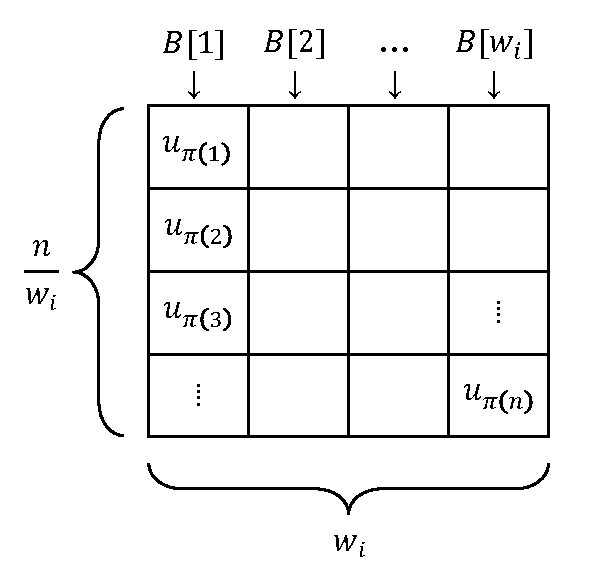
\includegraphics[width=0.7\linewidth]{images/matrices}
	\caption{Matrices generated by Algorithm~\ref{alg:Distribute} in round $i$}
	\label{fig:matrices}
\end{figure}

\begin{lemma} \label{lem:WhpMatrix}
	Let Algorithm~\ref{alg:MainSimple} call the modified version of \alg{Distribute} defined in Algorithm~\ref{alg:DistributeModified}, and ${m_i = 2^{i+1}}$ in each round $i$. Then, Algorithm~\ref{alg:MainSimple} guarantees that all honest users can connect to Tor with high probability, and the total number of bridges used is at most ${(6t - 1)c\log{n}}$.
\end{lemma}
\begin{proof}
	Since the $n$ users are arranged uniformly and independently at random in $M$, and there are $t_i$ active corrupt users among them, the probability that for a given user $u$ the column that $u$ appears in contains at least one corrupt user is at most
	\[1 - \left(\frac{n-t_i}{n}\right)^{\nicefrac{n}{m_i}} = 1 - \left(1-\frac{t_i}{n}\right)^{\nicefrac{n}{m_i}} \leq \frac{t_i}{m_i}.\]
	The last inequality is correct based on the Bernoulli's inequality when ${t_i \leq m_i}$. If ${b_i < 2^i}$, then ${t_i < 2^i}$ because in each round each corrupt user appears in exactly one column in $M$, and thus can block at most one bridge. Since in each round ${m_i = 2^{i+1} \geq 2t_i}$, this probability becomes a constant ${\leq 1/2}$.
	
	Since ${\lceil c\log{n} \rceil}$ instances of Algorithm~\ref{alg:MainSimple} run in parallel, the probability that every column that $u$ appears in among all matrices is ``bad'' (\ie, has at least one active corrupt user) is at most ${(1/2)^{c\log{n}} = 1/n^c}$.
	By applying the union bound, the probability that any of the $n$ users fails to sit in a ``good'' column (\ie, a column with no active corrupt user) is at most $1/n^{c-1}$. Therefore for any ${c > 1}$, all honest users can connect to Tor with high probability.	
	%	our choice of $m_i = 2^i$ in line~\ref{ln:DistributeSimple} of Algorithm~\ref{alg:MainSimple}, will eventually Since $c > 1$, it is sufficient to have $w_k \geq 2t_k$. Since the adversary's budget is bounded and $\frac{b_i}{ic\log{n}}$ is monotonically increasing, there exists some integer $k>0$ such that
	%	\[t_k \leq \frac{b_k}{kc\log{n}}.\]
	%	With our choice of $m_i = 2^i$ in line~\ref{ln:DistributeSimple} of Algorithm~\ref{alg:MainSimple}, we have
	%	\[t_k \leq \frac{b_k}{kc\log{n}} < \frac{k2^kc\log{n}}{kc\log{n}} = 2^k = w_k,\]
	%	which satisfies the condition $t_k < w_k$.
\end{proof}

\begin{figure*}
	\centering
	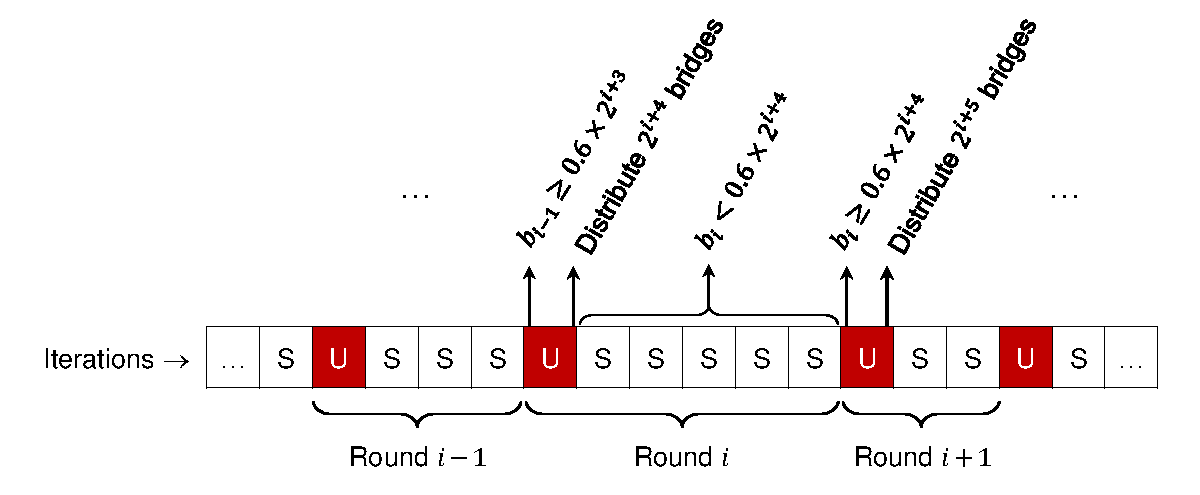
\includegraphics[width=0.76\linewidth]{images/rounds}
	\caption{Number of bridges distributed in the $i$-th round of Algorithm~\ref{alg:MainSimple}}
	\label{fig:rounds}
\end{figure*}

\begin{lemma} \label{lem:NumIterationsMatrix}
	By running Algorithm~\ref{alg:MainSimple}, all honest users can connect to Tor with high probability after at most ${\lceil \log{t} \rceil + 1}$ iterations.
\end{lemma}
\begin{proof}
	Similar to Lemma~\ref{lem:NumIterationsBasic}, we let $k$ denote the smallest number of rounds needed until all users can connect to Tor with high probability. $k$ is bounded, because $t$ is bounded. So, for all ${i \geq k}$, ${b_i < 2^i}$, and based on Lemma~\ref{lem:WhpMatrix}, all users can connect to Tor with high probability. We now find $k$ with respect to $t$. 
	
	In each round $i$, the adversary can maximize $k$ by minimizing the number of bridges blocked (\ie, $b_i$), while ensuring the algorithm proceeds to the next round. This can be done by blocking only half of the $2^{i+1}$ bridges distributed in each round and memorizing the rest $2^{i}$ bridge addresses to be blocked in future rounds, where ${t < 2^i}$. Let $\ell$ be the smallest integer such that ${t \leq 2^\ell}$.
	Until round $\ell$, the adversary can memorize at most 
	\[\sum_{j=1}^{\ell-1} 2^j = 2^{\ell} - 2\] 
	bridges. In round $\ell$, no more bridges can be memorized, because the adversary has to block all of the ${t \leq 2^\ell}$ bridges it has learned in this round to force the algorithm to proceed to round ${\ell + 1}$.  In round ${\ell + 1}$, however, the adversary can block at most 
	\[2^\ell - 2 + 2^\ell = 2^{\ell+1} - 2 < 2^{\ell+1}\] 
	bridges, which is insufficient for proceeding to round ${\ell + 2}$. Therefore, ${\ell + 1}$ is the last round and ${k = \ell + 1}$. Since ${t \leq 2^\ell}$, ${k = \lceil \log{t} \rceil + 1}$. In other words, if the algorithm is run for at least ${\lceil \log{t} \rceil + 1}$ iterations, then all honest users succeed with high probability.	
	%	For any $i \leq k$, consider the algorithm in three consecutive rounds $i - 1$, $i$, and $i+1$ as shown in Figure~\ref{fig:rounds}. In round $i-1$, the algorithm proceeds to line~\ref{ln:ConditionSimple}, where only one of the following two cases is possible:
	%	\begin{enumerate}
	%		\item \label{case:whp} $b_{i-1} < 2^{i-1}$: Based on Lemma~\ref{lem:whpSimple}, all honest users can connect to Tor with high probability.
	%		
	%		\item $b_{i-1} \geq 2^{i-1}$: The algorithm proceeds to the next round (round $i$) and distributes $w_{i} = 2^{i+1}$ bridges. Consider the following two possible cases:
	%		\begin{enumerate}
	%			\item $i < k$: In order for the algorithm to proceed to the next round, the adversary has to block at least $2^i$ bridges, otherwise Case~\ref{case:whp} happens and all honest users can connect to Tor with high probability. The adversary can memorize the remainder at most $2^i$ bridge addresses to block in future rounds.
	%			
	%			\item $i = k$: Since this is the last round, the adversary can only block less than half of the $2^{k+1}$ bridges distributed in this round. In fact, it can block at most $t$ bridges learned from the current round as well as \[\sum_{j=1}^{k-2} 2^j = 2^{k-1} - 2\] bridges learned (but not blocked) from the previous rounds. Therefore, we find $k$ sufficiently large such that $2^k > t + 2^{k-1} - 2$. This results in $k > \log{(t-2)} + 1$.
	%		\end{enumerate}
	%	\end{enumerate}
	%	Thus, if the algorithm is run for at least $\lfloor\log{(t-2)}\rfloor + 2 = O(\log{t})$ iterations, then with high probability all honest users are guaranteed to be able to connect to Tor.
\end{proof}

\begin{lemma} \label{lem:NumBridgesMatrix}
	The total number of bridges used by Algorithm~\ref{alg:DistributeModified} is at most ${(12t - 2)c\log{n}}$.
\end{lemma}
\begin{proof}
	Similar to Lemma~\ref{lem:NumBridgesBasic}, the total number of bridges can be calculated from~\eqref{eq:NumBridges}.
	In the $i$-th round, the algorithm recruits ${a_i \leq 2^{i+1}}$ new bridges. Since ${b_i < 2^i}$,
	\[N_i < 2^{i+1} + \sum_{j=1}^{i-1} 2^j = 2^{i+1} + 2^{i} - 2 = 3 \cdot 2^i - 2.\]
	
	From Lemma~\ref{lem:NumIterationsMatrix}, it is sufficient to run the algorithm for ${\lceil \log{t} \rceil + 1}$ rounds. Hence,
	\[N_i < 3 \cdot 2^{\lceil \log{t} \rceil + 1} - 2 < 12t - 2,\]
	\ie, the total number of bridges used by the algorithm is at most ${(12t - 2)c\log{n}}$.
\end{proof}

In the following lemma, we use martingales to show that the number of bridges used by the algorithm can be reduced by a factor of two when a constant fraction of the users are corrupted, \ie, when ${t = \alpha n}$, for some constant ${\alpha \in [0,1]}$. To achieve this, we let Algorithm~\ref{alg:MainSimple} distribute only ${m_i = 2^i}$ bridges in each round.

\begin{lemma} \label{lem:azumaMatrix}
	Let only a fixed constant fraction of the users be corrupted, and ${m_i = 2^i}$ in each round $i$ of Algorithm~\ref{alg:MainSimple}. The algorithm guarantees all honest users can connect to Tor with high probability, and the total number of bridges used is ${(8t - 2)c\log{n}}$.
\end{lemma}
\begin{proof}
	For $j=1,2,...,m_i$, let $\{X_j\}$ be a sequence of random variables each corresponding to the $j$-th column of $M$, where each column consists of $\frac{n}{m_i}$ users chosen uniformly at random without replacement from the set of all users. Also, let $Y$ be a random variable corresponding to the number of columns that have no corrupt users. Since $\E[|Y|] < \infty$, the sequence $\{Z_j = \E[Y|X_1,...,X_j]\}$ defines a Doob martingale. Since the probability that a given column has no corrupt user is at least $\left((n-t_i)/n\right)^{n/m_i}$, by the linearity of expectation, \[\E[Y] = m_i \cdot \left(1-\frac{t_i}{n}\right)^{\nicefrac{n}{m_i}}.\]
	Since in each round ${m_i = 2^i \geq t_i}$ and ${t = \alpha n}$, for some constant ${\alpha \in [0,1]}$, we have ${\E[Y] = m_i(1-\alpha)^{1/\alpha}}$. This means that, in expectation, a constant fraction of the columns in each matrix (in each round) are good.
	Since choosing one random column changes the expected number of good columns by at most one, ${|Z_{j+1} - Z_j| \leq 1}$. Using the Azuma's inequality, we get 
	\[\Pr\left(|Y-\E[Y]|\right) \geq \lambda) \leq 2e^{\nicefrac{-2\lambda^2}{m_i}},\] 
	for any ${\lambda > 0}$.
	Therefore, the actual values of $Y$ are highly concentrated around its expected value $\E[Y]$.
	
	The number of bridges distributed in each round of the modified algorithm is ${m_i=2^i}$. Thus, using equation~\eqref{eq:NumBridges} in Lemma~\ref{lem:NumBridgesBasic}, the total number of bridges used by the modified algorithm is at most ${(8t - 2)c\log{n}}$.
\end{proof}

\subsection{Detection Scheme} \label{sec:Fixed}
In this section, we describe a technique for detecting and blacklisting corrupt users which allows us to reduce the number of bridges used by the algorithm from $O(t\log{n})$ to $O(t)$.

\begin{algorithm}[H]
	\caption{Bridge Distribution with Detection Scheme}
	\label{alg:MainFixed}
	
	\vspace{2pt}
	\algFont \vspace{5pt}
	\begin{algorithmic}[1]
		\State Initialize parameters: $c > 0$; $i \gets 1$; $U \gets$ a set of users $\{u_1,...,u_{n}\}$
		\State \Call{Distribute}{$2,c,U$} %\Comment{Distribute $2c\log{n}$ real bridges}
		\State \Call{DistributeFakes}{$c,U$} %\Comment{Distribute $nc\log{n}$ fake bridges}
		
		\While{\True}
			\State $b_i \gets$ number of real bridges blocked so far %\Comment{Using~\cite{Ensafi:2014:DIP:2722265.2722279}}
			
			\State From $U$, delete every user whom any of the fake 
			\Statex \hspace{\algorithmicindent}bridges assigned to it is blocked
			\If {$b_i \geq i2^ic\log{n}$} \label{ln:ConditionFixed}
				\State $i \gets i+1$ \label{ln:IncrementFixed}  %\Comment{Proceed to the next round}
				\State \Call{Distribute}{$2^i,c,U$} \label{ln:DistributeFixed} %\Comment{Distribute $2^ic\log{n}$ real bridges}
				\State \Call{DistributeFakes}{$c,U$} %\Comment{Distribute $nc\log{n}$ fake bridges}
			\EndIf
		\EndWhile
	\end{algorithmic}
\end{algorithm}

\begin{algorithm}
	\caption{Fake Bridge Distribution}
	\label{alg:DistFakes}
	
	\algFont \vspace{5pt}
	\textit{Goal:} A set of $nc\log{n}$ fake bridges is distributed among a set of $n$ users $U = \{u_1,...,u_n\}$.
	\begin{algorithmic}[1]
		\Function{DistributeFakes}{$U$}
			\State Initialize parameter: $n \gets |U|$; $F \gets$ a list of 
			\Statex \hspace{\algorithmicindent}$cn\log{n}$ unblocked fake bridges
			\ForAll{$j \in [n]$} %\Comment{Assign $c\log{n}$ fake bridges to each user}
				\State Assign $F[(j-1)c\log{n} + 1],...,F[jc\log{n}]$ to $u_j$
			\EndFor
		\EndFunction
	\end{algorithmic}
\end{algorithm}

\subsubsection{Proof of Algorithm~\ref{alg:MainFixed}} \label{sec:ProofFixed}

PAGES 47-50 OF THE HANDNOTES

\subsection{Sublinear Bridge Cost}
In Algorithm~\ref{alg:MainFixed}, we assume each iteration is either successful or unsuccessful. Then, we show that $O(t\log{t}\log{n})$ bridges are needed to ensure that we get at least one successful iteration among $O(\log{t})$ iterations. Unfortunately, this algorithm and the corresponding analysis do not consider the number of honest users whom have been assigned at least one unblocked bridge even in unsuccessful iterations. In this section, we introduce a slightly modified model, where in the beginning of the algorithm, each user is holding one message to send to Tor. The goal is to guarantee that at the end of the algorithm, each user is given at least one chance to send its message to Tor. In other words, we guarantee that each user is given at least one unblocked bridge before the algorithm terminates.

\begin{algorithm}[H]
	\caption{Bridge Distribution Scheme}
	\label{alg:MainFinal}
	
	\algFont \vspace{2pt}
	\begin{algorithmic}[1]
		\State Initialize parameters: $c > 0$; $i \gets 1$; $U \gets$ a set of users $\{u_1,...,u_{n_i}\}$; $n_i \gets |U|$
		\State \Call{Distribute}{$2,c, U$} %\Comment{Distribute $2c\log{n}$ unblocked bridges}
		\While{$n_i > 0$}
			\State $b_i \gets$ number of bridges blocked so far %\Comment{Using~\cite{Ensafi:2014:DIP:2722265.2722279}}

			\If {$b_i \geq i2^ic\log{n_i}$} \label{ln:ConditionFinal}
				\State $i \gets i+1$ \label{ln:IncrementFinal} %\Comment{Proceed to the next round}
				\ForAll{$k \in [c\log{n}]$}
					\State \Call{DistributeSingles}{$2^i, c, U$} \label{ln:DistributeFinal} %\Comment{Distribute $2^ic\log{n}$ unblocked bridges}
				\EndFor
			\EndIf
			\State From $U$, remove the users that have successfully sent their message
			\State $n_i \gets |U|$ %\Comment{Update the number of users}			
		\EndWhile
	\end{algorithmic}
\end{algorithm}

\begin{algorithm}
	\caption{Randomized Real/Fake Bridge Distribution}
	\label{alg:DistributeFinal}
	
	\algFont \vspace{5pt}
	\textit{Goal:} A set of $w$ real bridges and $n$ fake bridges is randomly distributed among a set of $n$ users $U = \{u_1,...,u_n\}$.
	\begin{algorithmic}[1]
		\Function{DistributeSingles}{$w,c,U$}
			\State Initialize parameter: $n \gets |U|$; $B \gets$ a list of $wc\log{n}$ unblocked bridges \label{ln:recruitBridgesFinal}
			\State Define a matrix $M$ with $w$ columns and $\frac{n}{w}$ rows such that for all $i \in [\frac{n}{w}]$ and $j \in [w]$, we
			\Statex \hspace{\algorithmicindent}have $M_{i,j} = [u_{j + (i-1)w}]$. \label{ln:defMatricesFinal}
			
			\State $r \gets$ a sequence of $\Theta(n\log{n})$ bits chosen uniformly and independently at random
			\State $M \gets$ \alg{Shuffle($r, M$)}
			\ForAll{$j \in [w]$}
				\ForAll{$i \in [\frac{n}{w}]$}
					\State $x \gets$ a value chosen randomly from $[0,1]$
					\If{$x \leq p$}
						\State Assign $B[j + (k-1)w]$ to the user in $M_{i,j}$ 	\label{ln:assignColumnsFinal}
					\Else
						\State Assign a fake bridge to the user in $M_{i,j}$
					\EndIf
				\EndFor
			\EndFor
		\EndFunction
	\end{algorithmic}
\end{algorithm}

\subsection{Proof of Algorithm~\ref{alg:MainFinal}} \label{sec:ProofFinal}
PAGES 55-58 OF THE HANDNOTES

\subsection{Multi-Distributor Model}

\begin{figure*}[t]
	\centering
	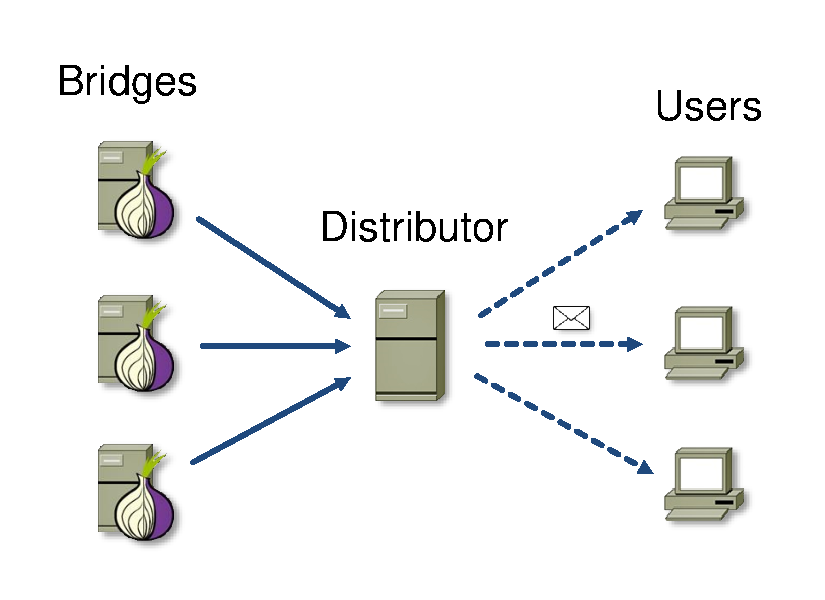
\includegraphics[width=0.47\linewidth]{images/single-alg}
	\hspace{2.2em}
	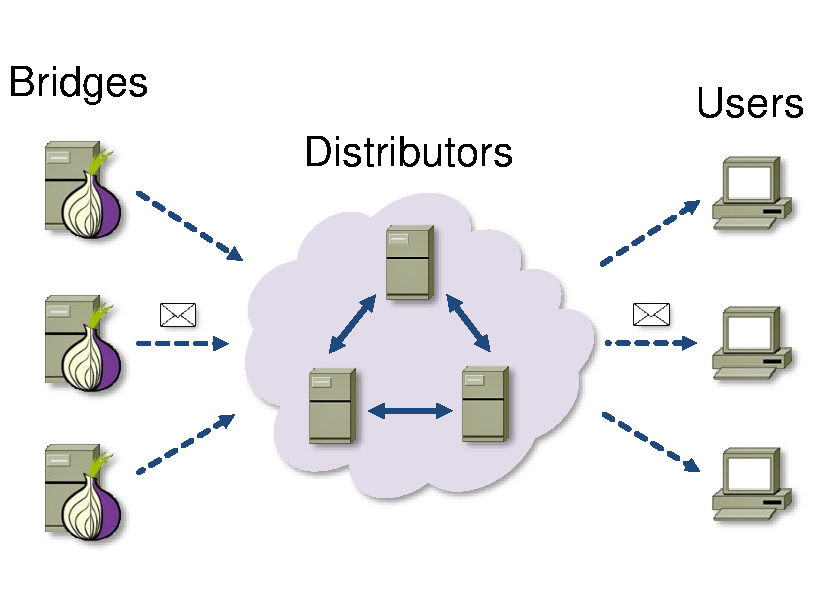
\includegraphics[width=0.47\linewidth]{images/multi-alg}
	\caption{Our single-distributor (left) and multi-distributor (right) algorithms}
	\label{fig:model}
\end{figure*}

\section{Evaluation} \label{sec:simulations}
To evaluate various properties of our algorithms, we implemented a proof-of-concept prototype and tested it in a simulated environment under various adversarial behavior. The prototype is written in C\# using .NET Framework 4.5. We ran the simulations on an Intel Core i5-4250U 1.3GHz machine with 4GB of RAM running Windows 10 Pro. We set the parameters of our protocols in such a way that we ensure the failure probability of the distribution algorithm is smaller than $10^{-5}$.

\begin{figure*}[tbph]
	\hspace{-0.8em}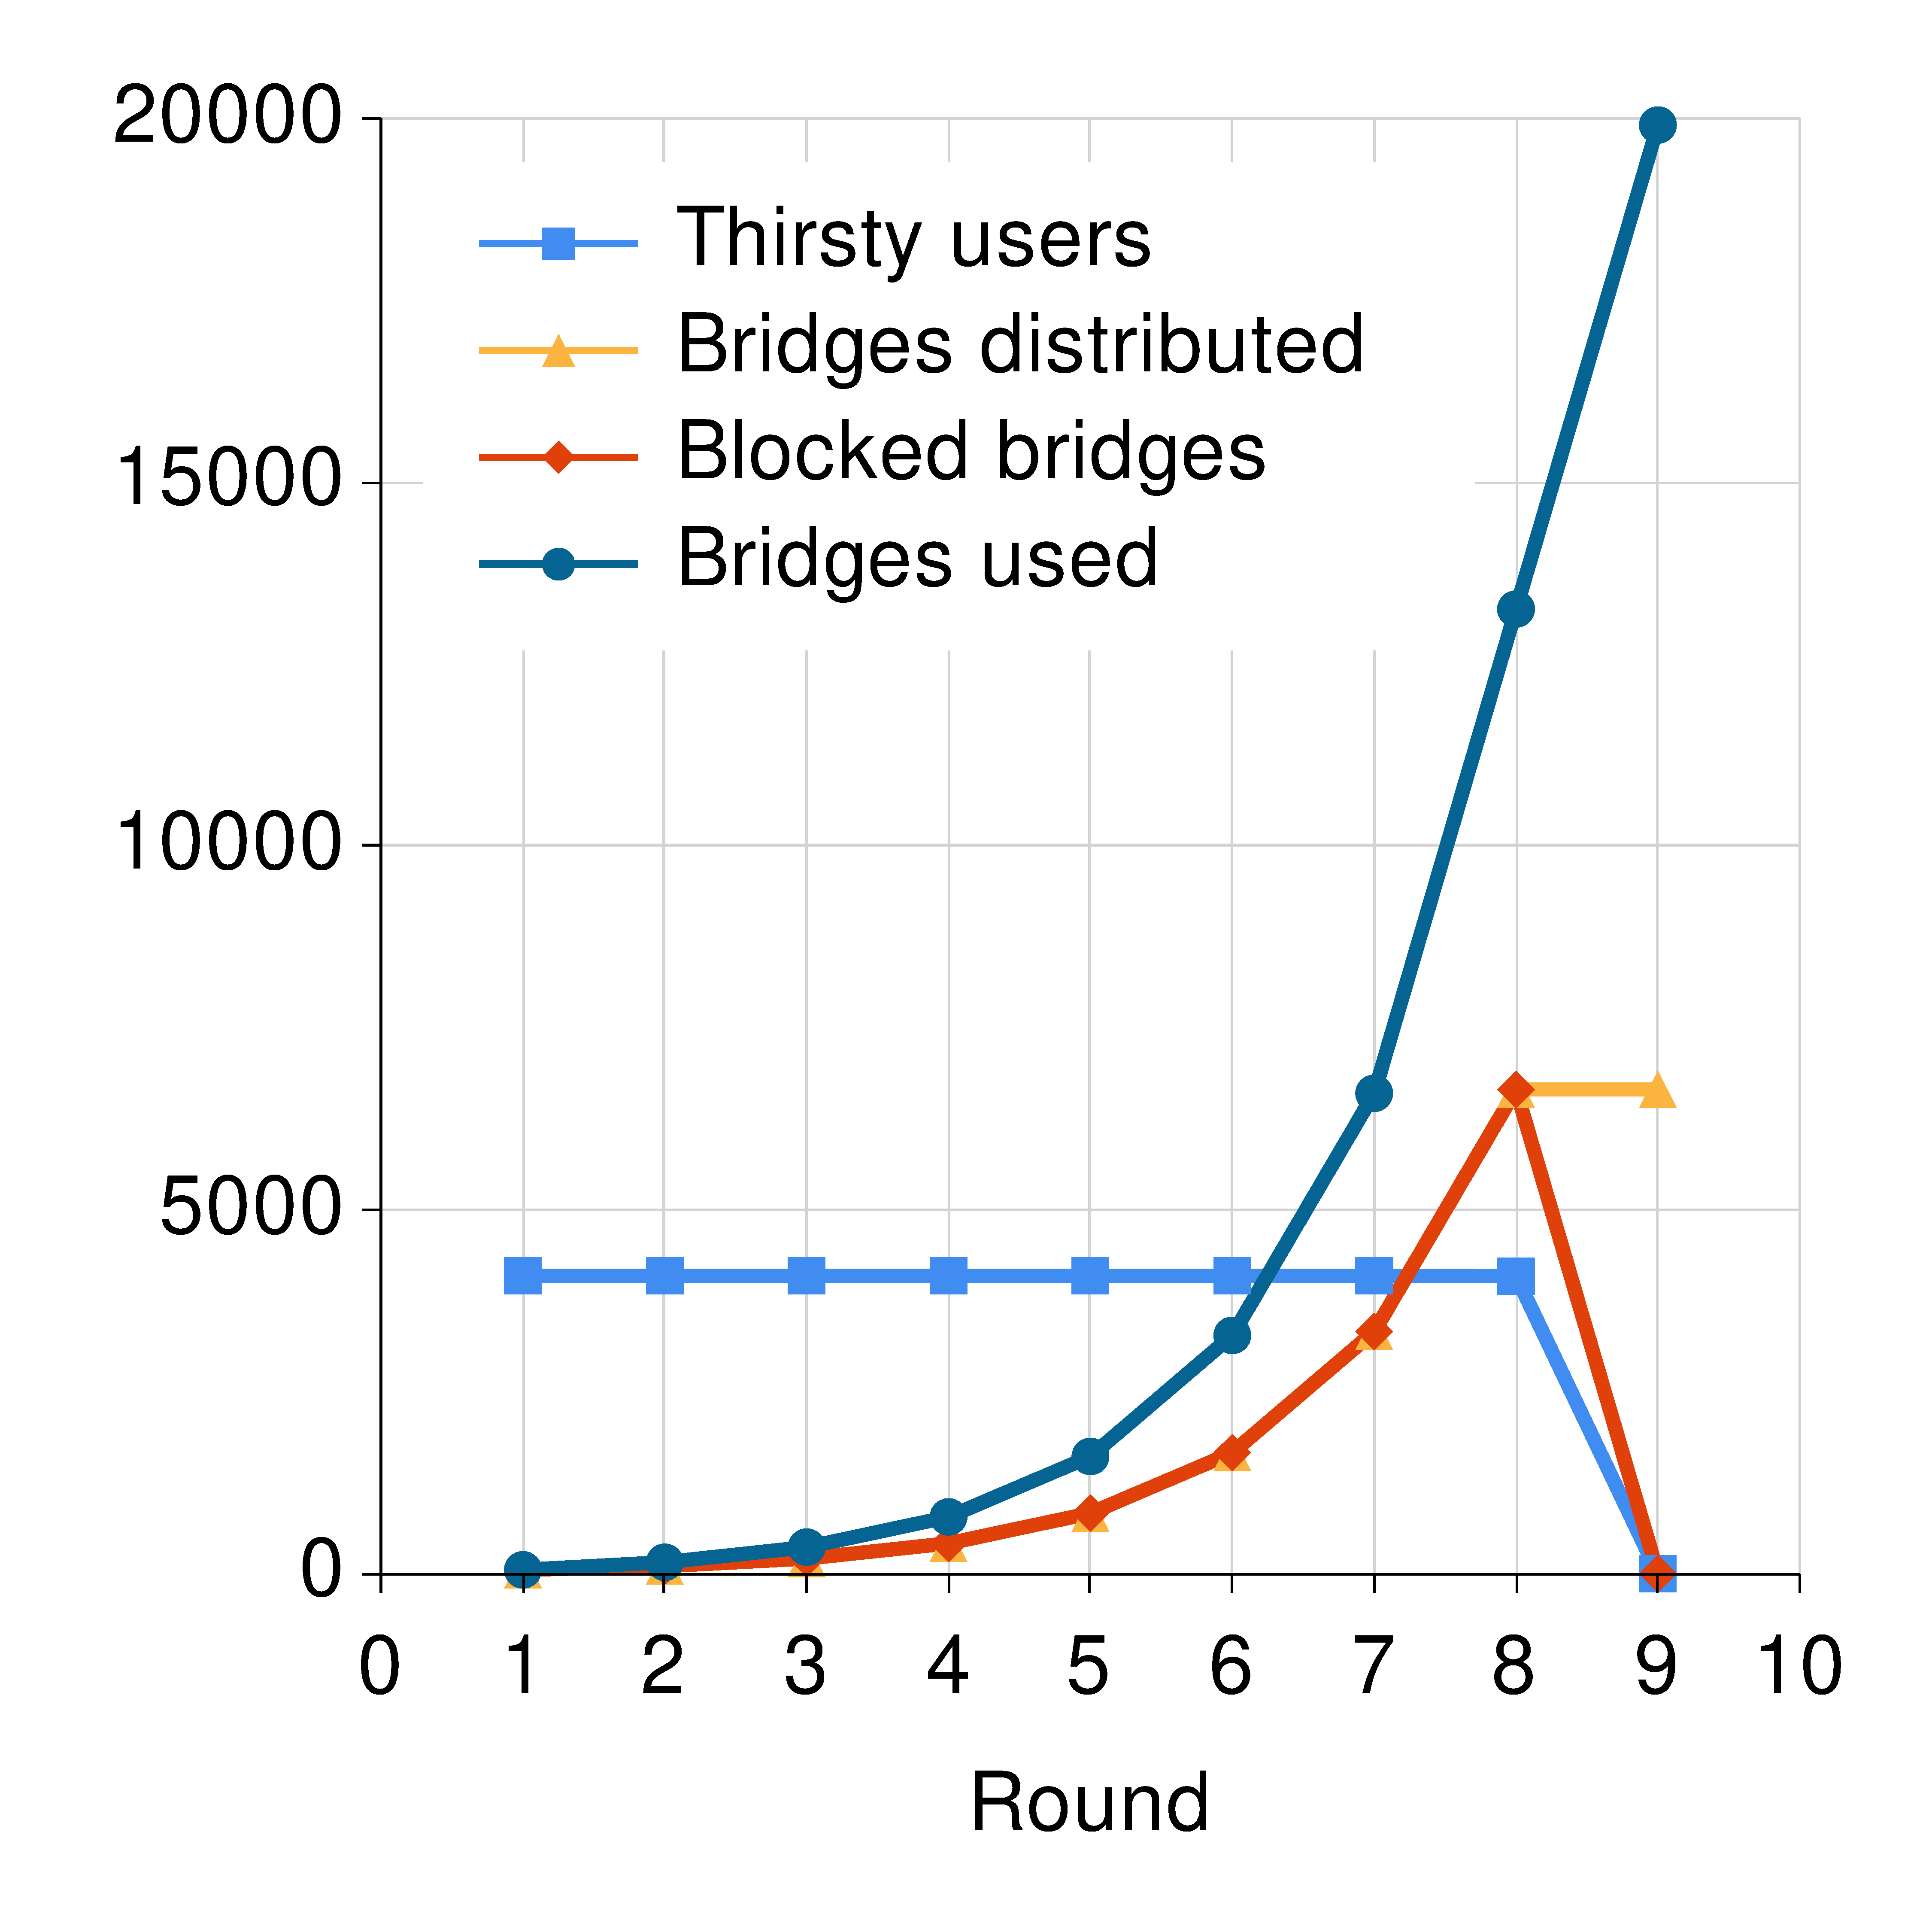
\includegraphics[width=0.35\textwidth]{images/plot-aggressive-8192}\hspace{-0.5em}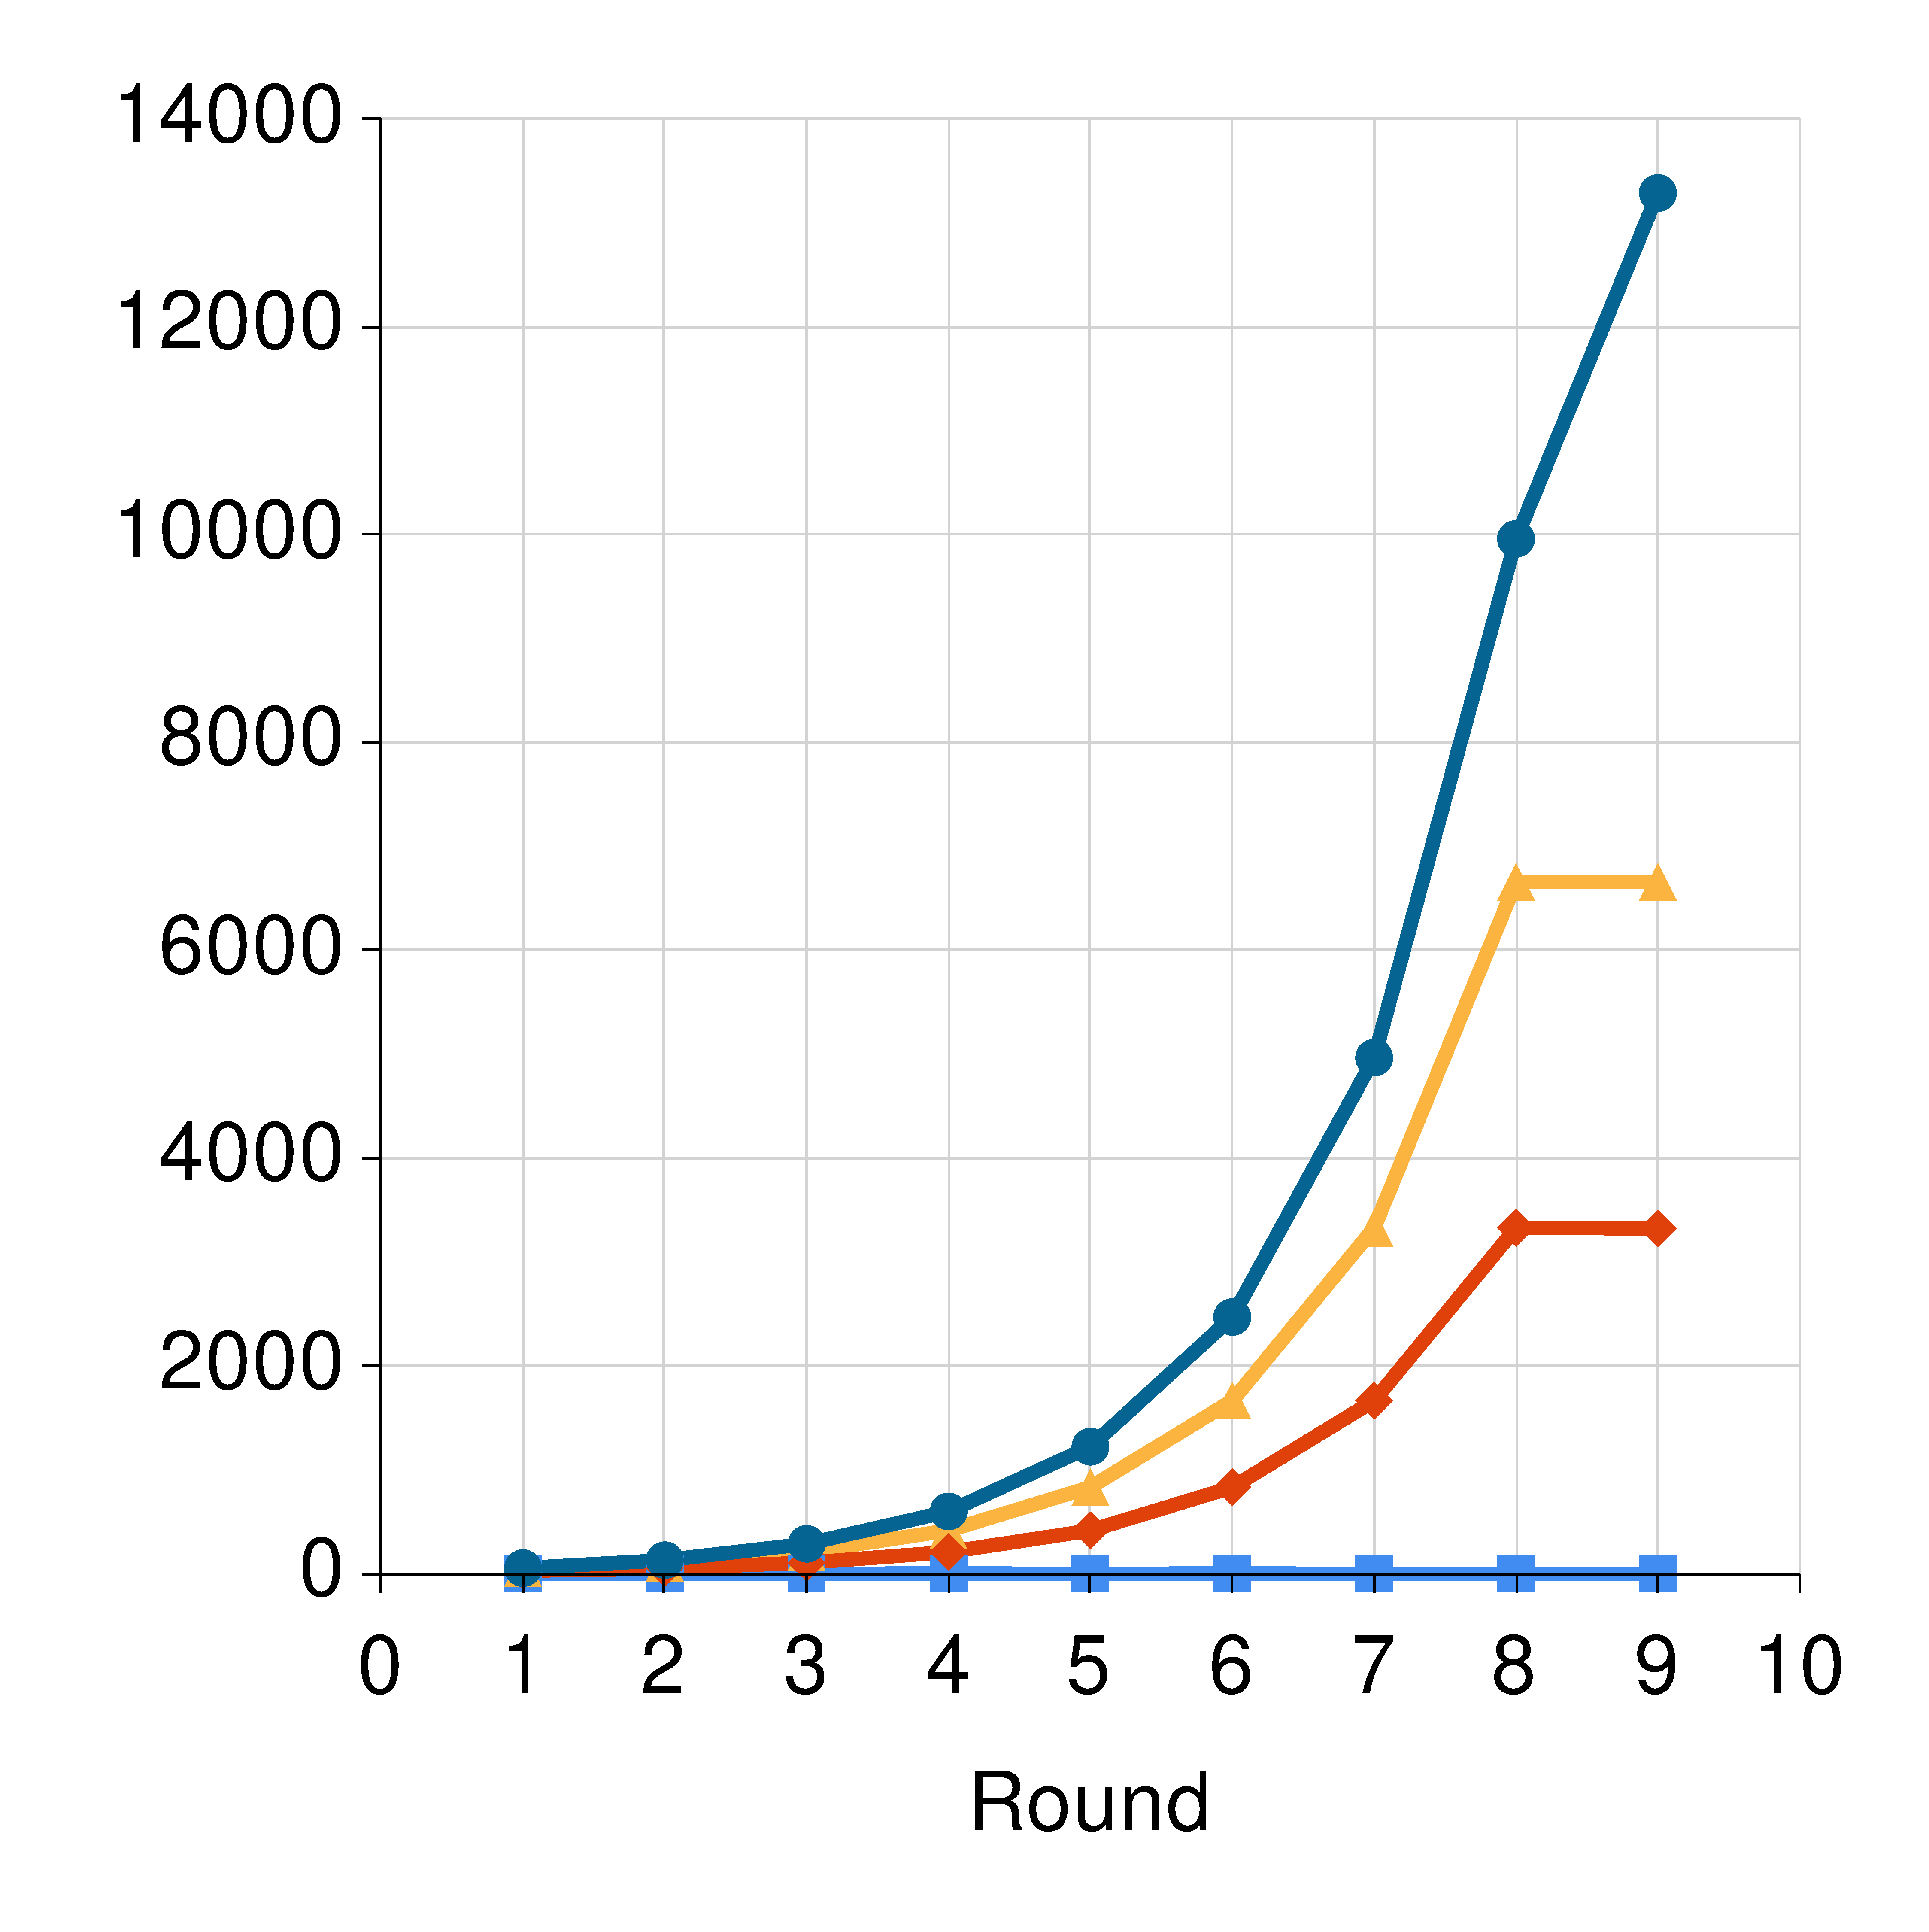
\includegraphics[width=0.35\textwidth]{images/plot-prudent-8192}\hspace{-0.5em}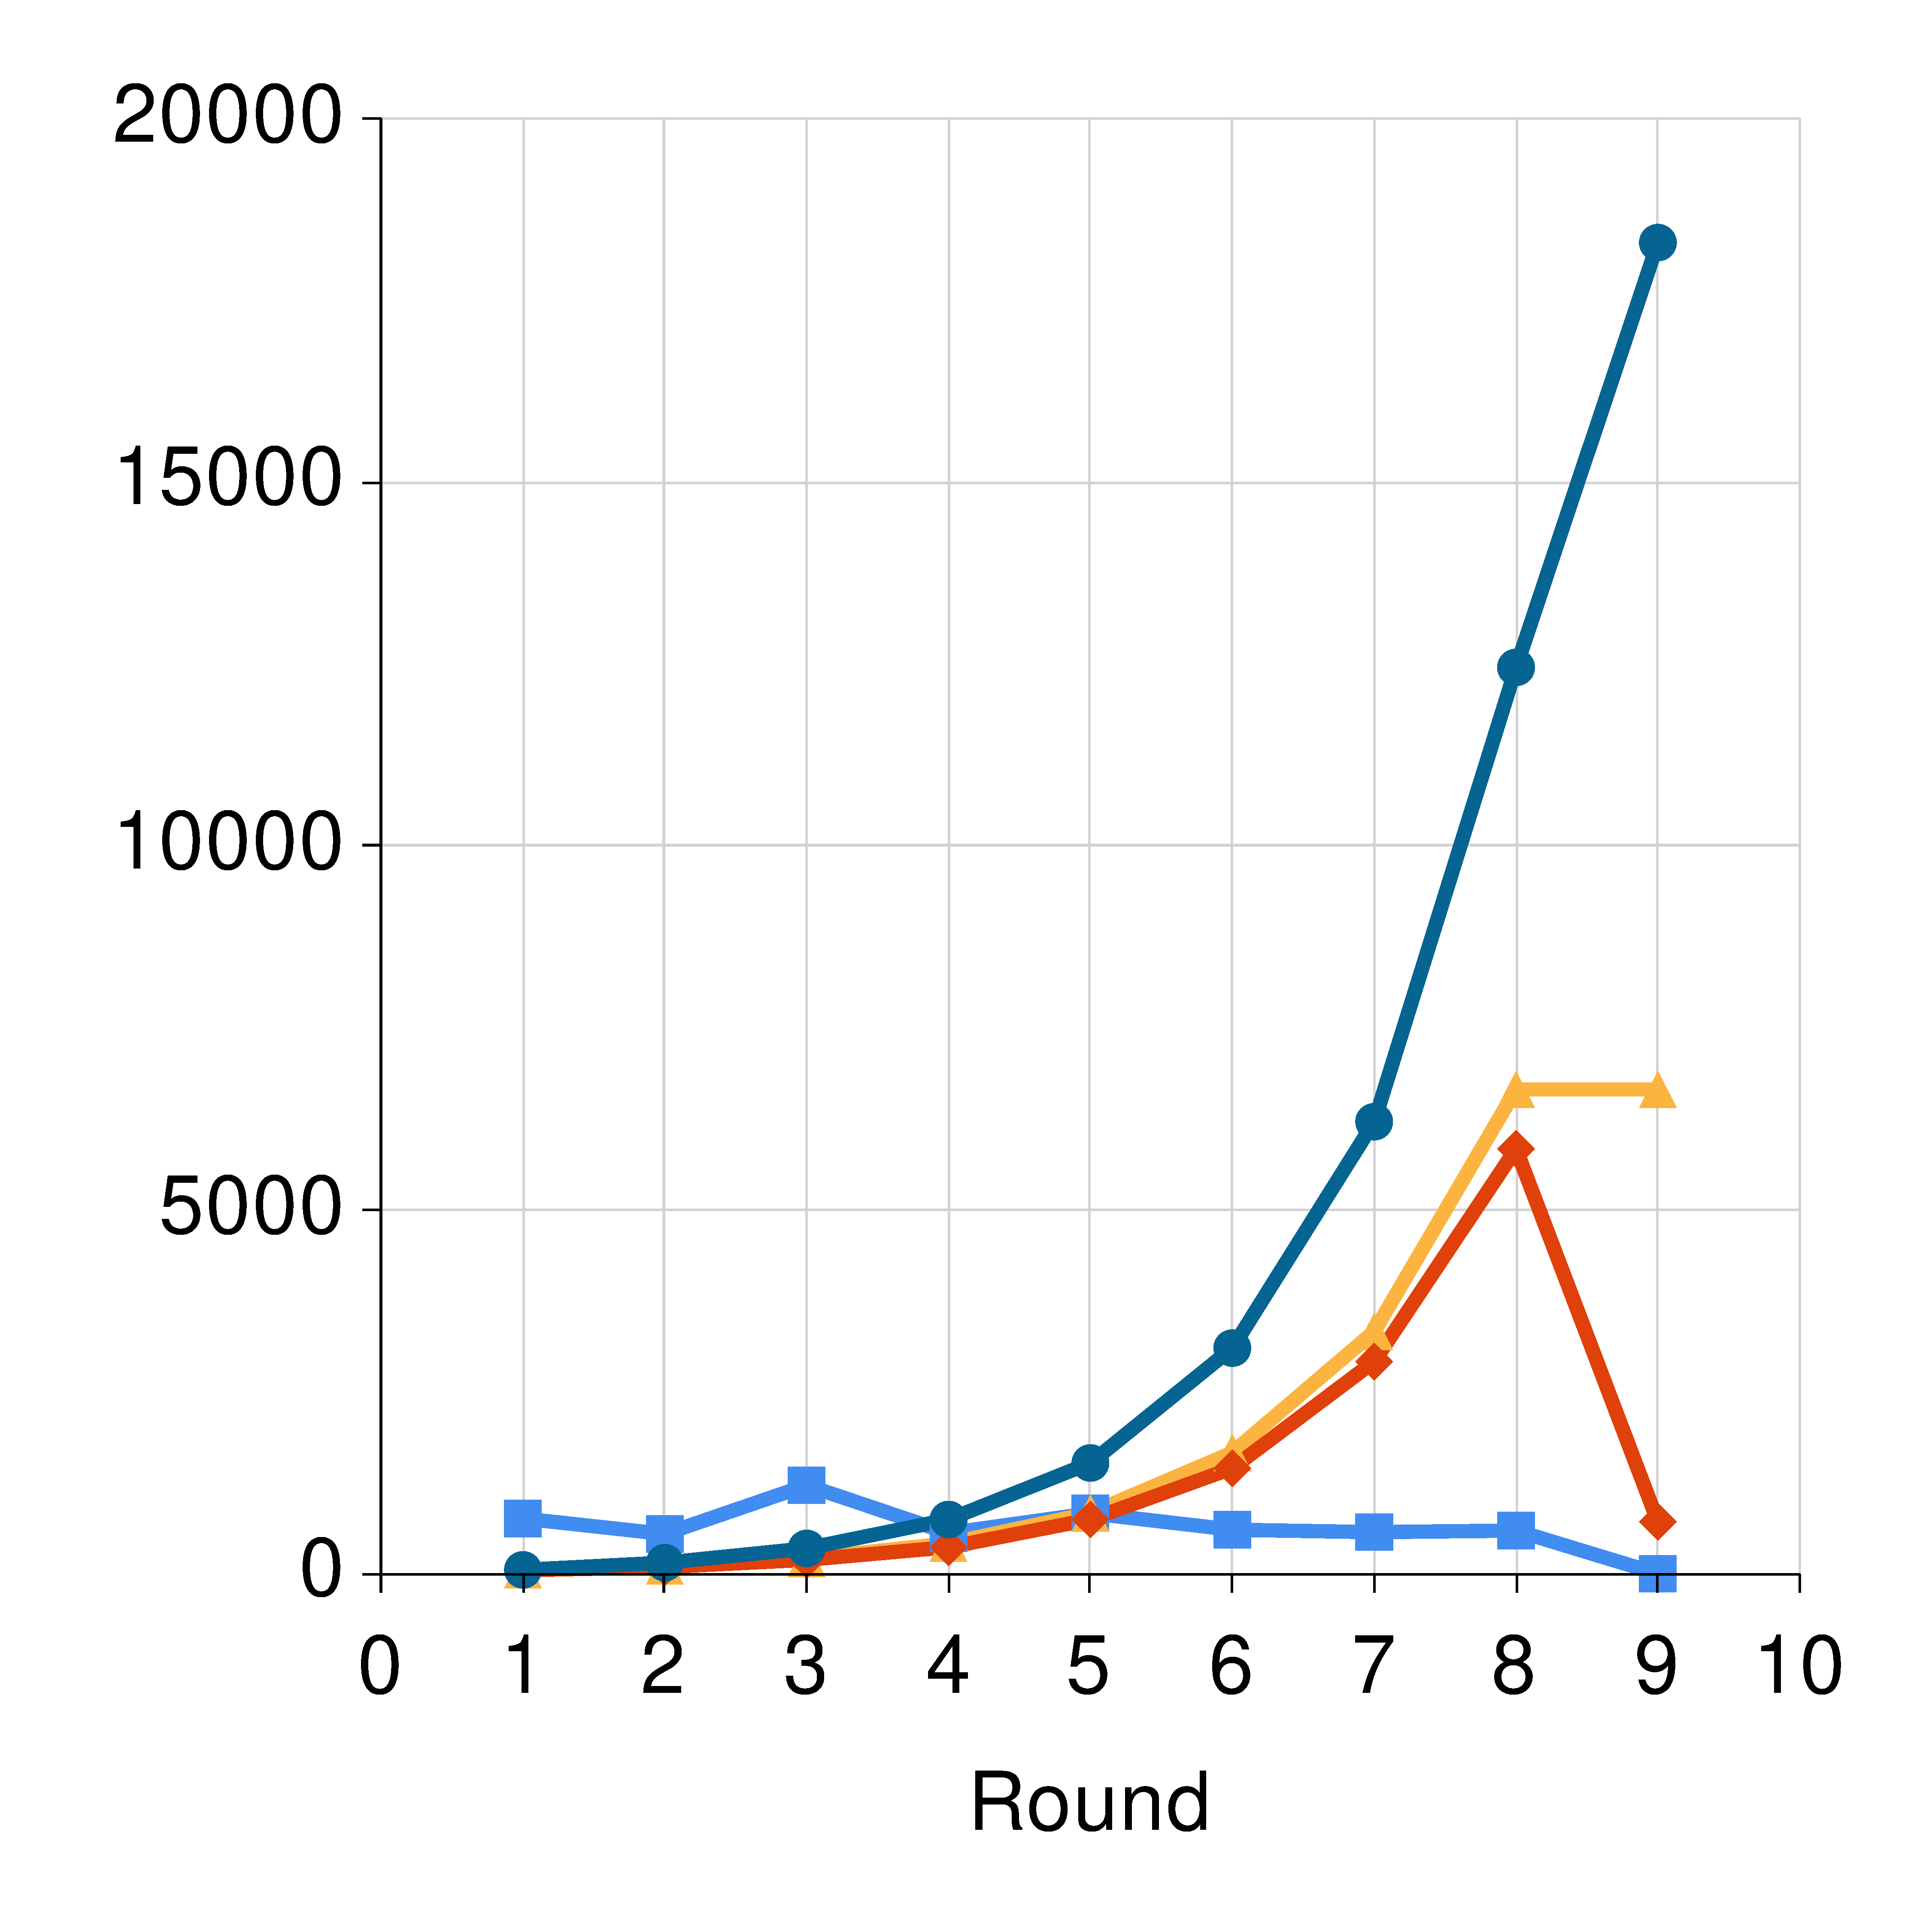
\includegraphics[width=0.35\textwidth]{images/plot-stochastic-8192}\caption{Simulation results for $n=8192$ and $t=4096$ with aggressive (left)
		prudent (middle), and stochastic (right) adversary.}
	\label{fig:circuit-1} 
\end{figure*}

\begin{figure*}[tbph]
	\hspace{-0.8em}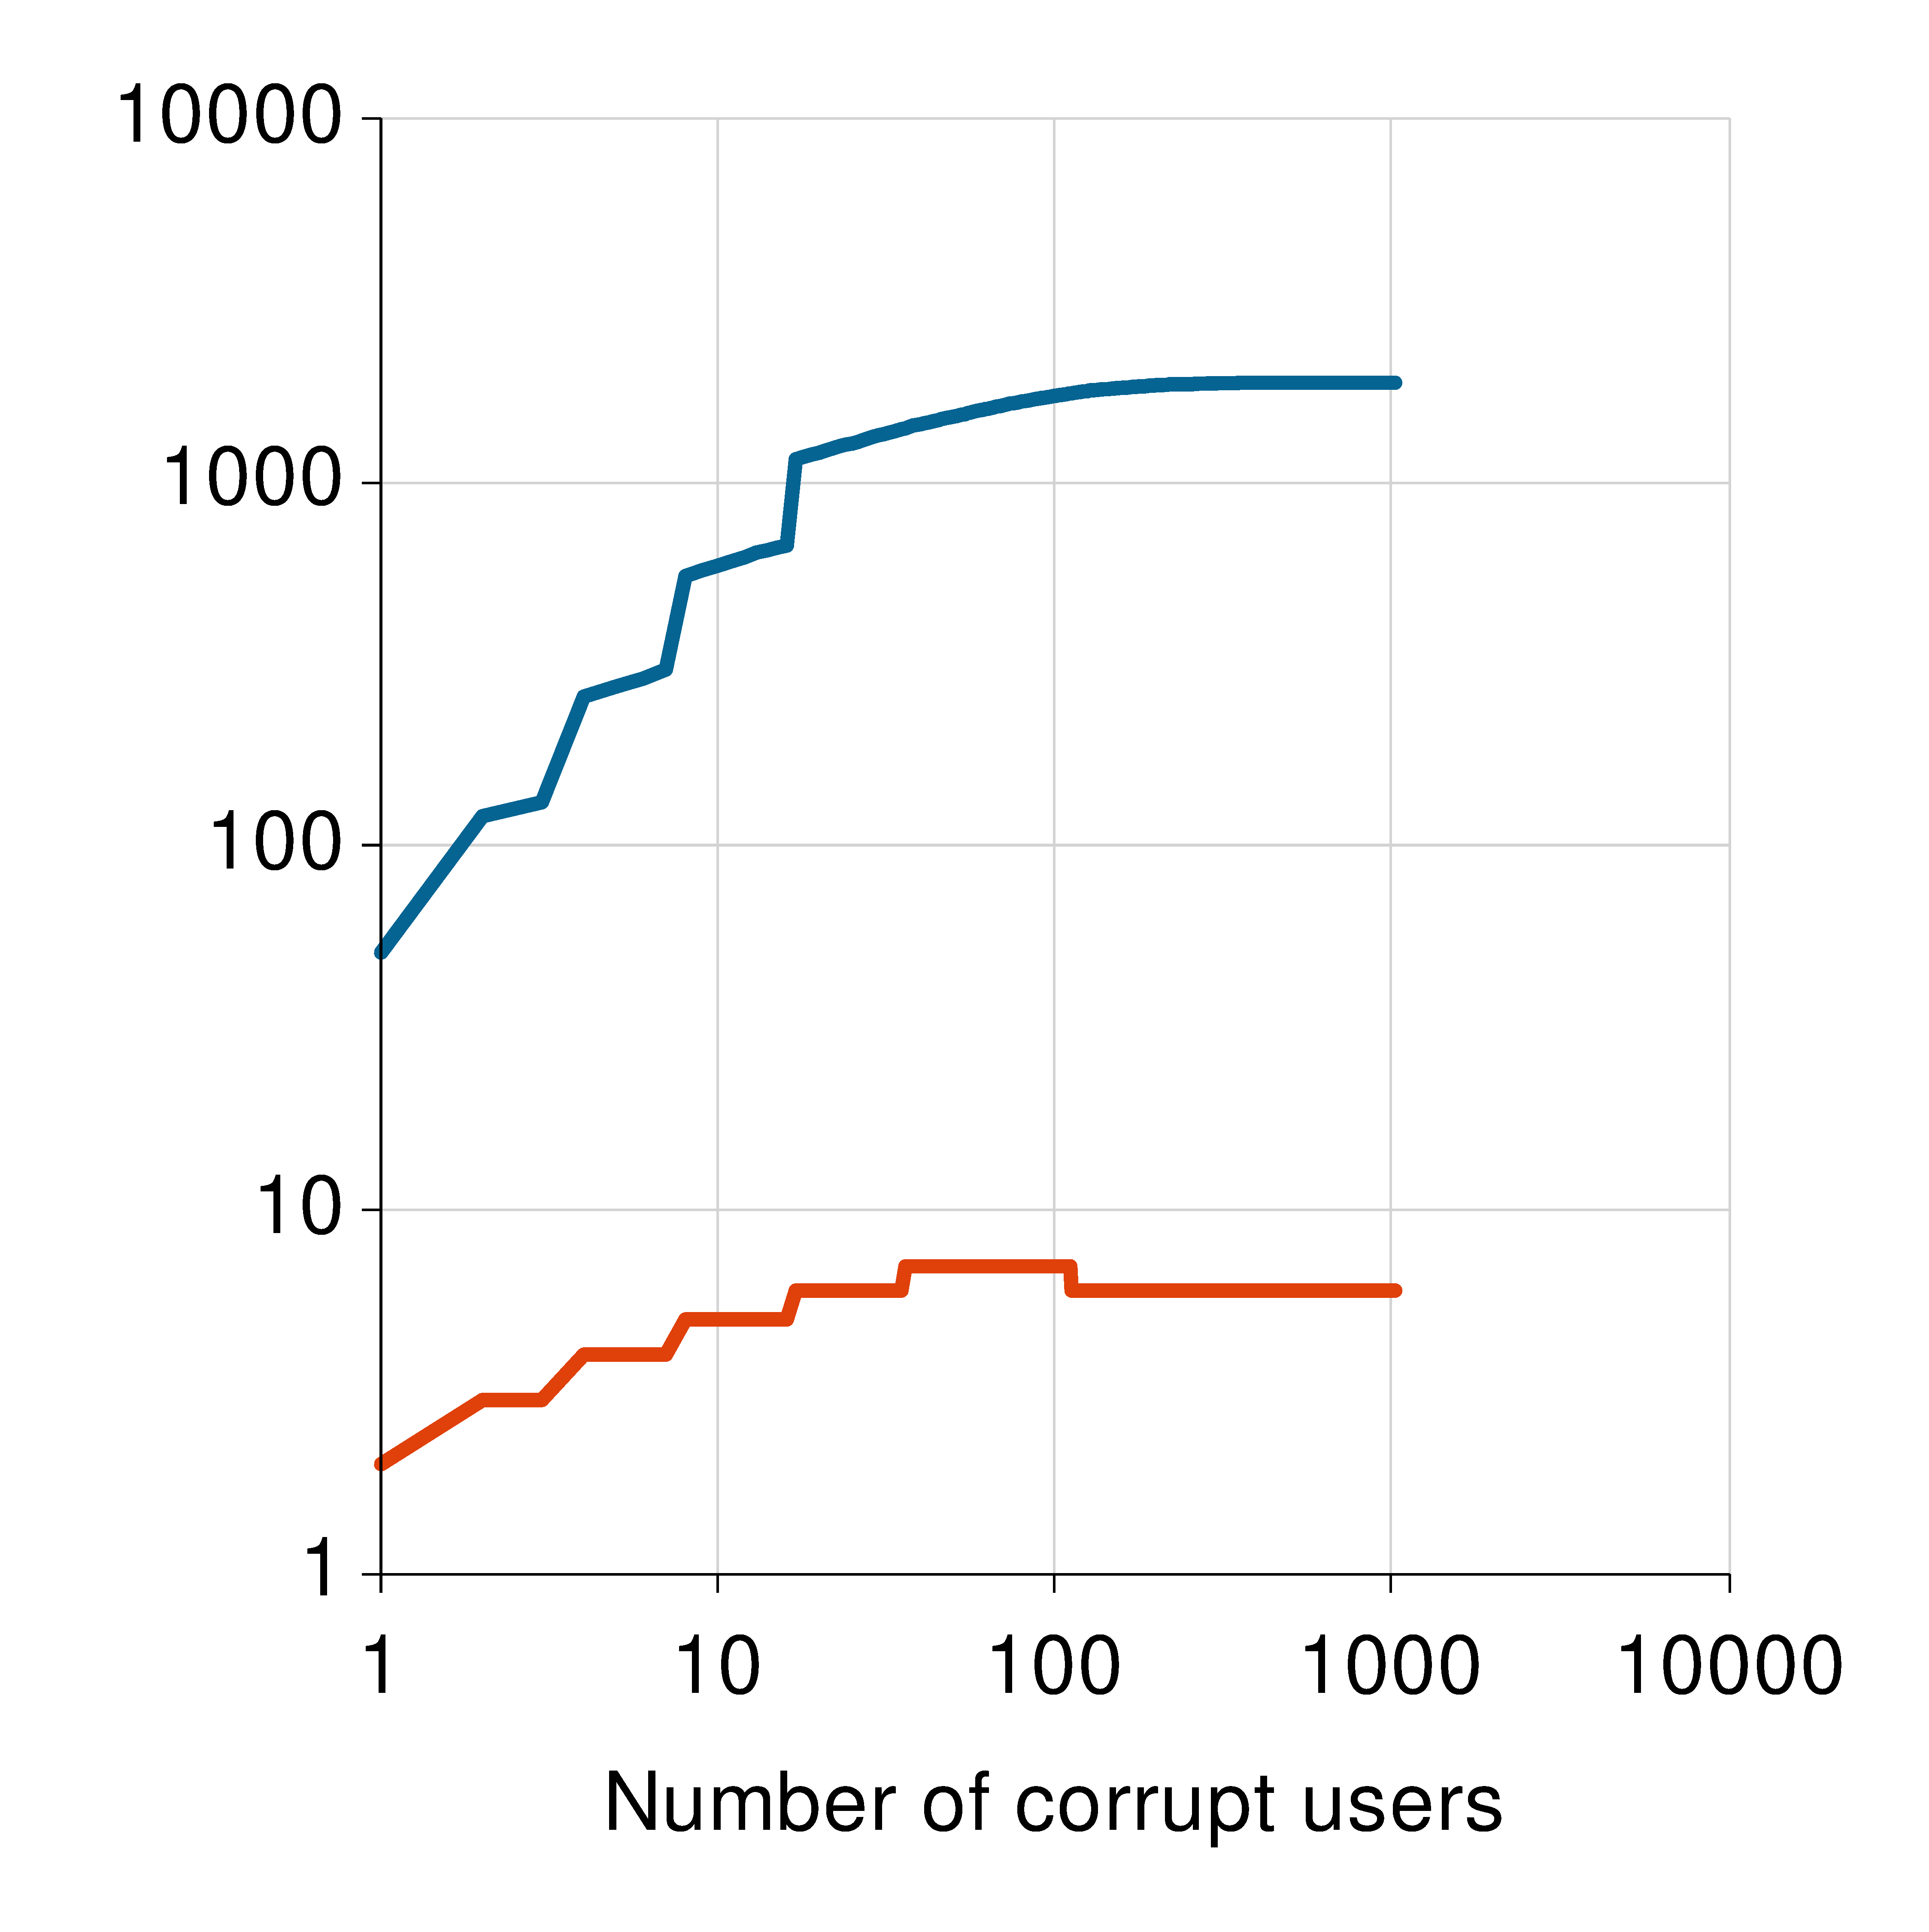
\includegraphics[width=0.35\textwidth]{images/plot-aggressive-VarT-1024}\hspace{-0.5em}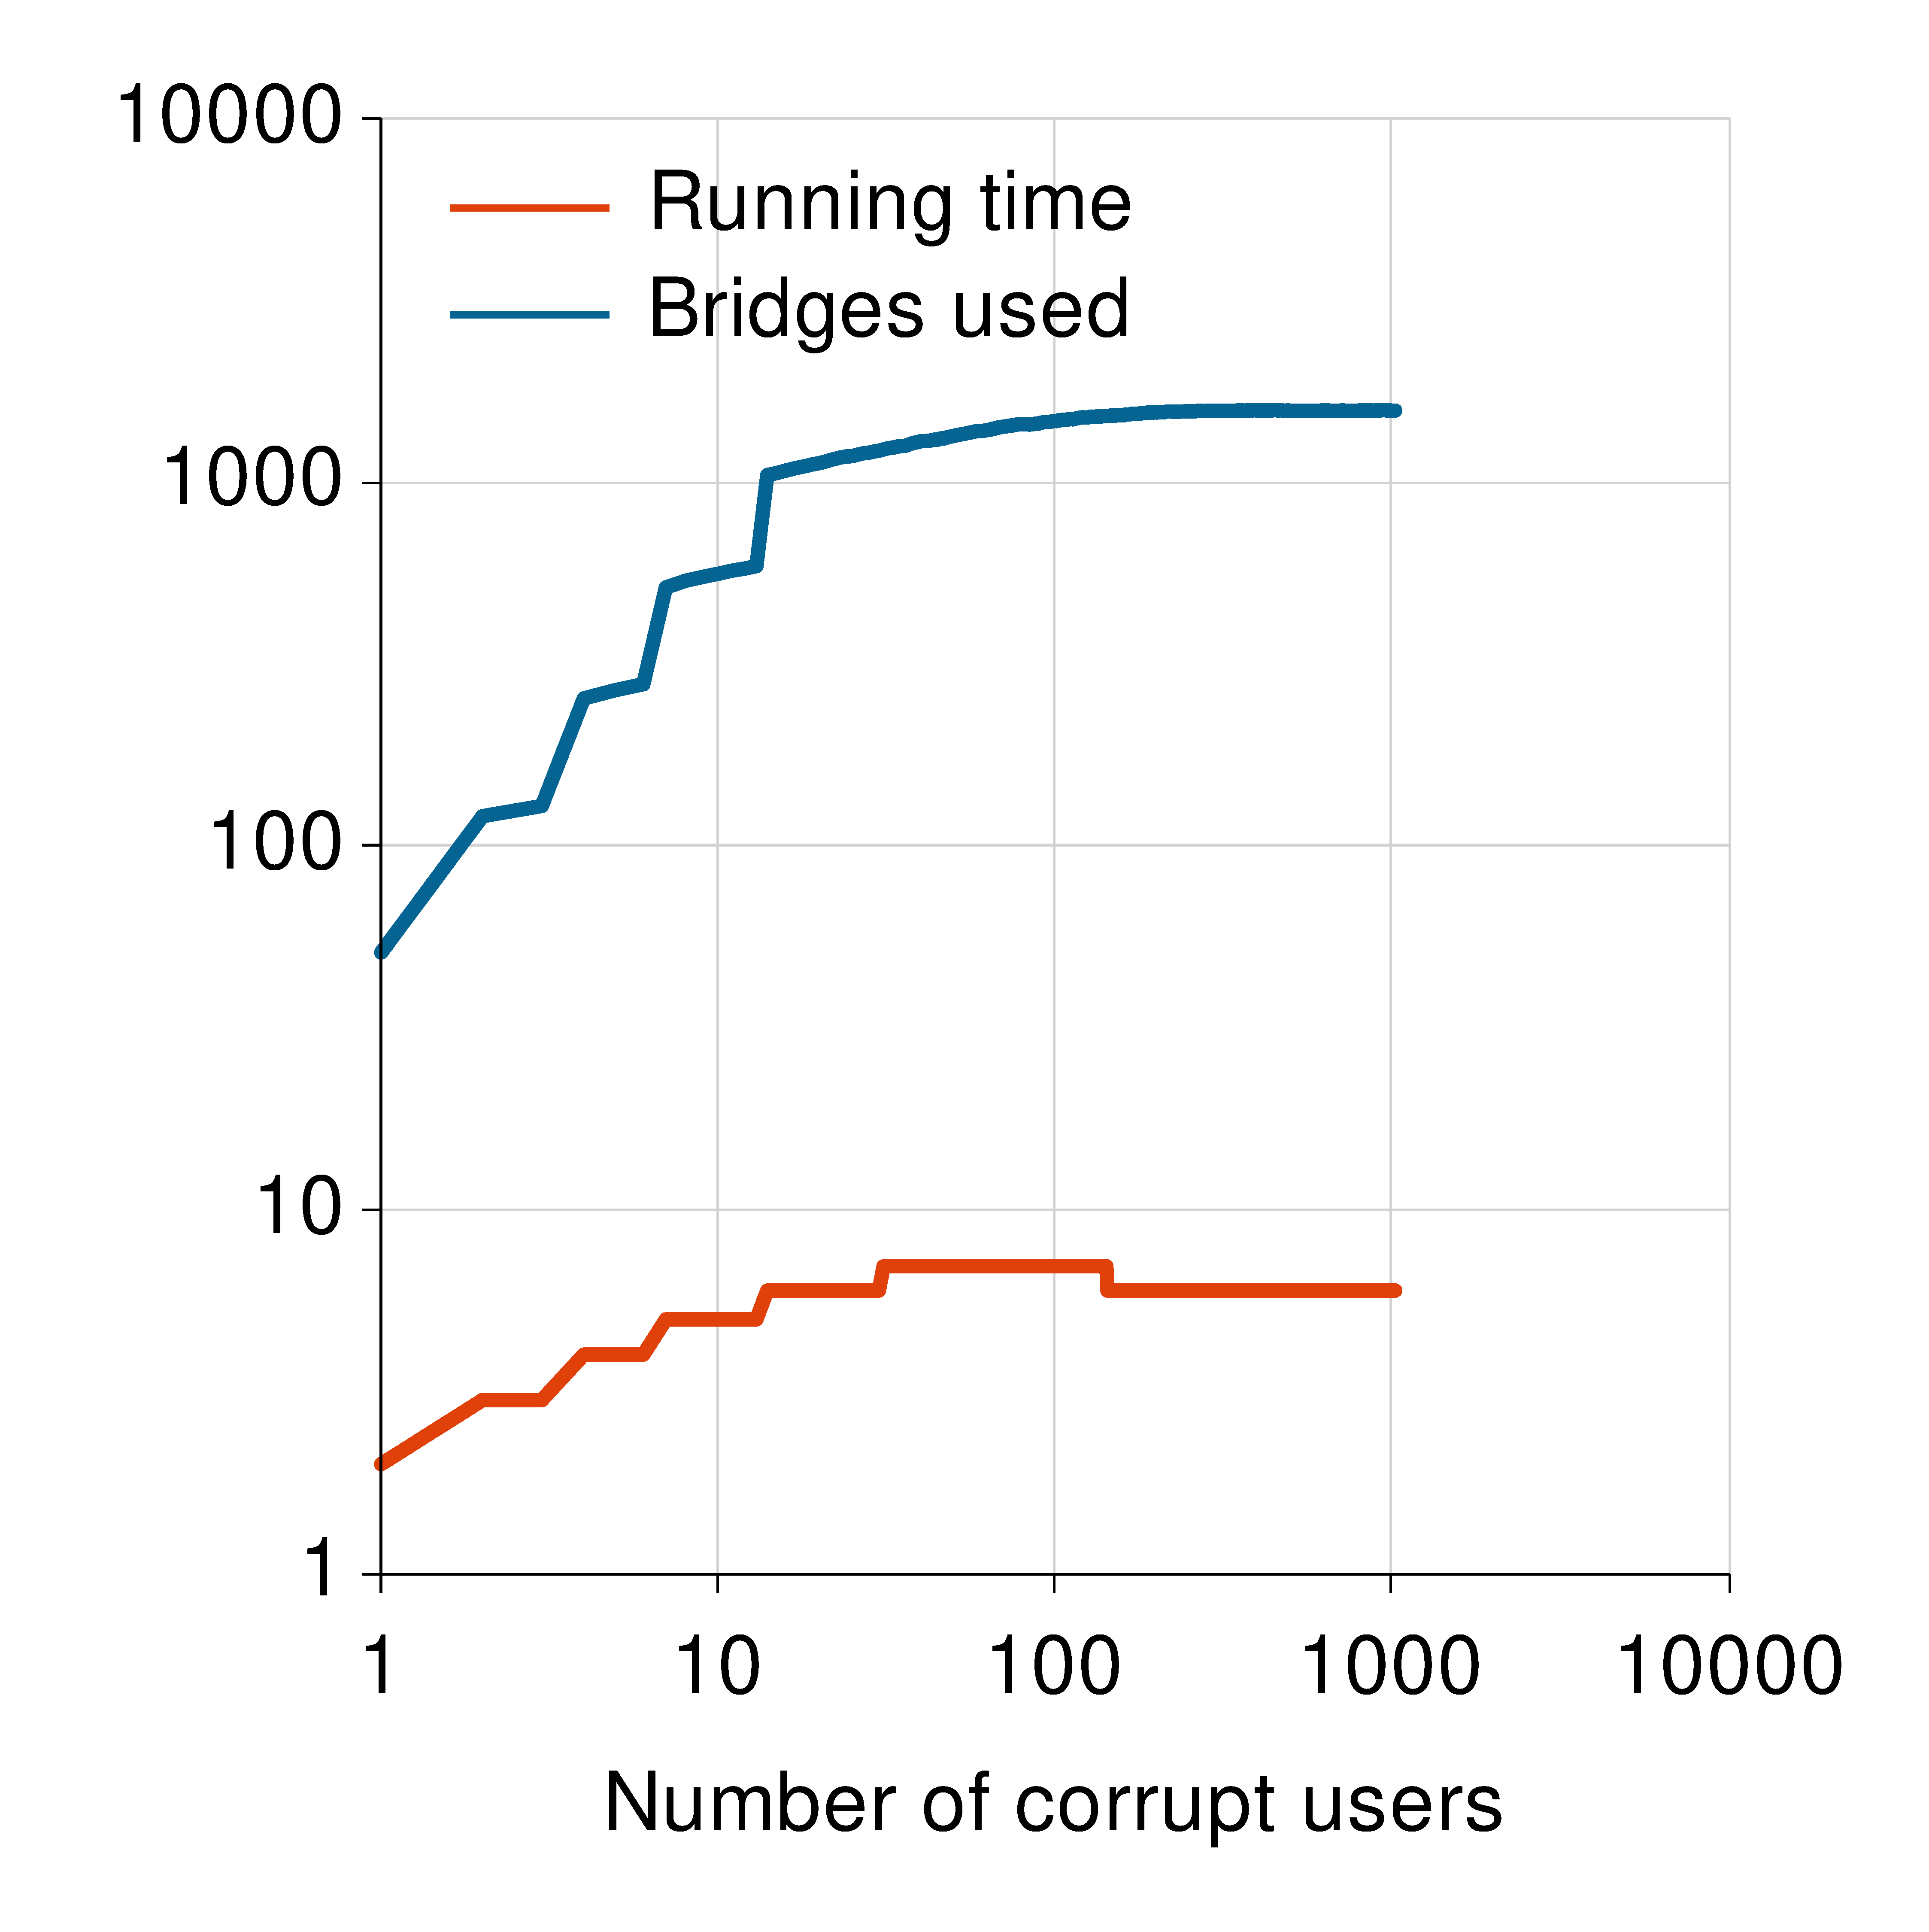
\includegraphics[width=0.35\textwidth]{images/plot-prudent-VarT-1024}\hspace{-0.5em}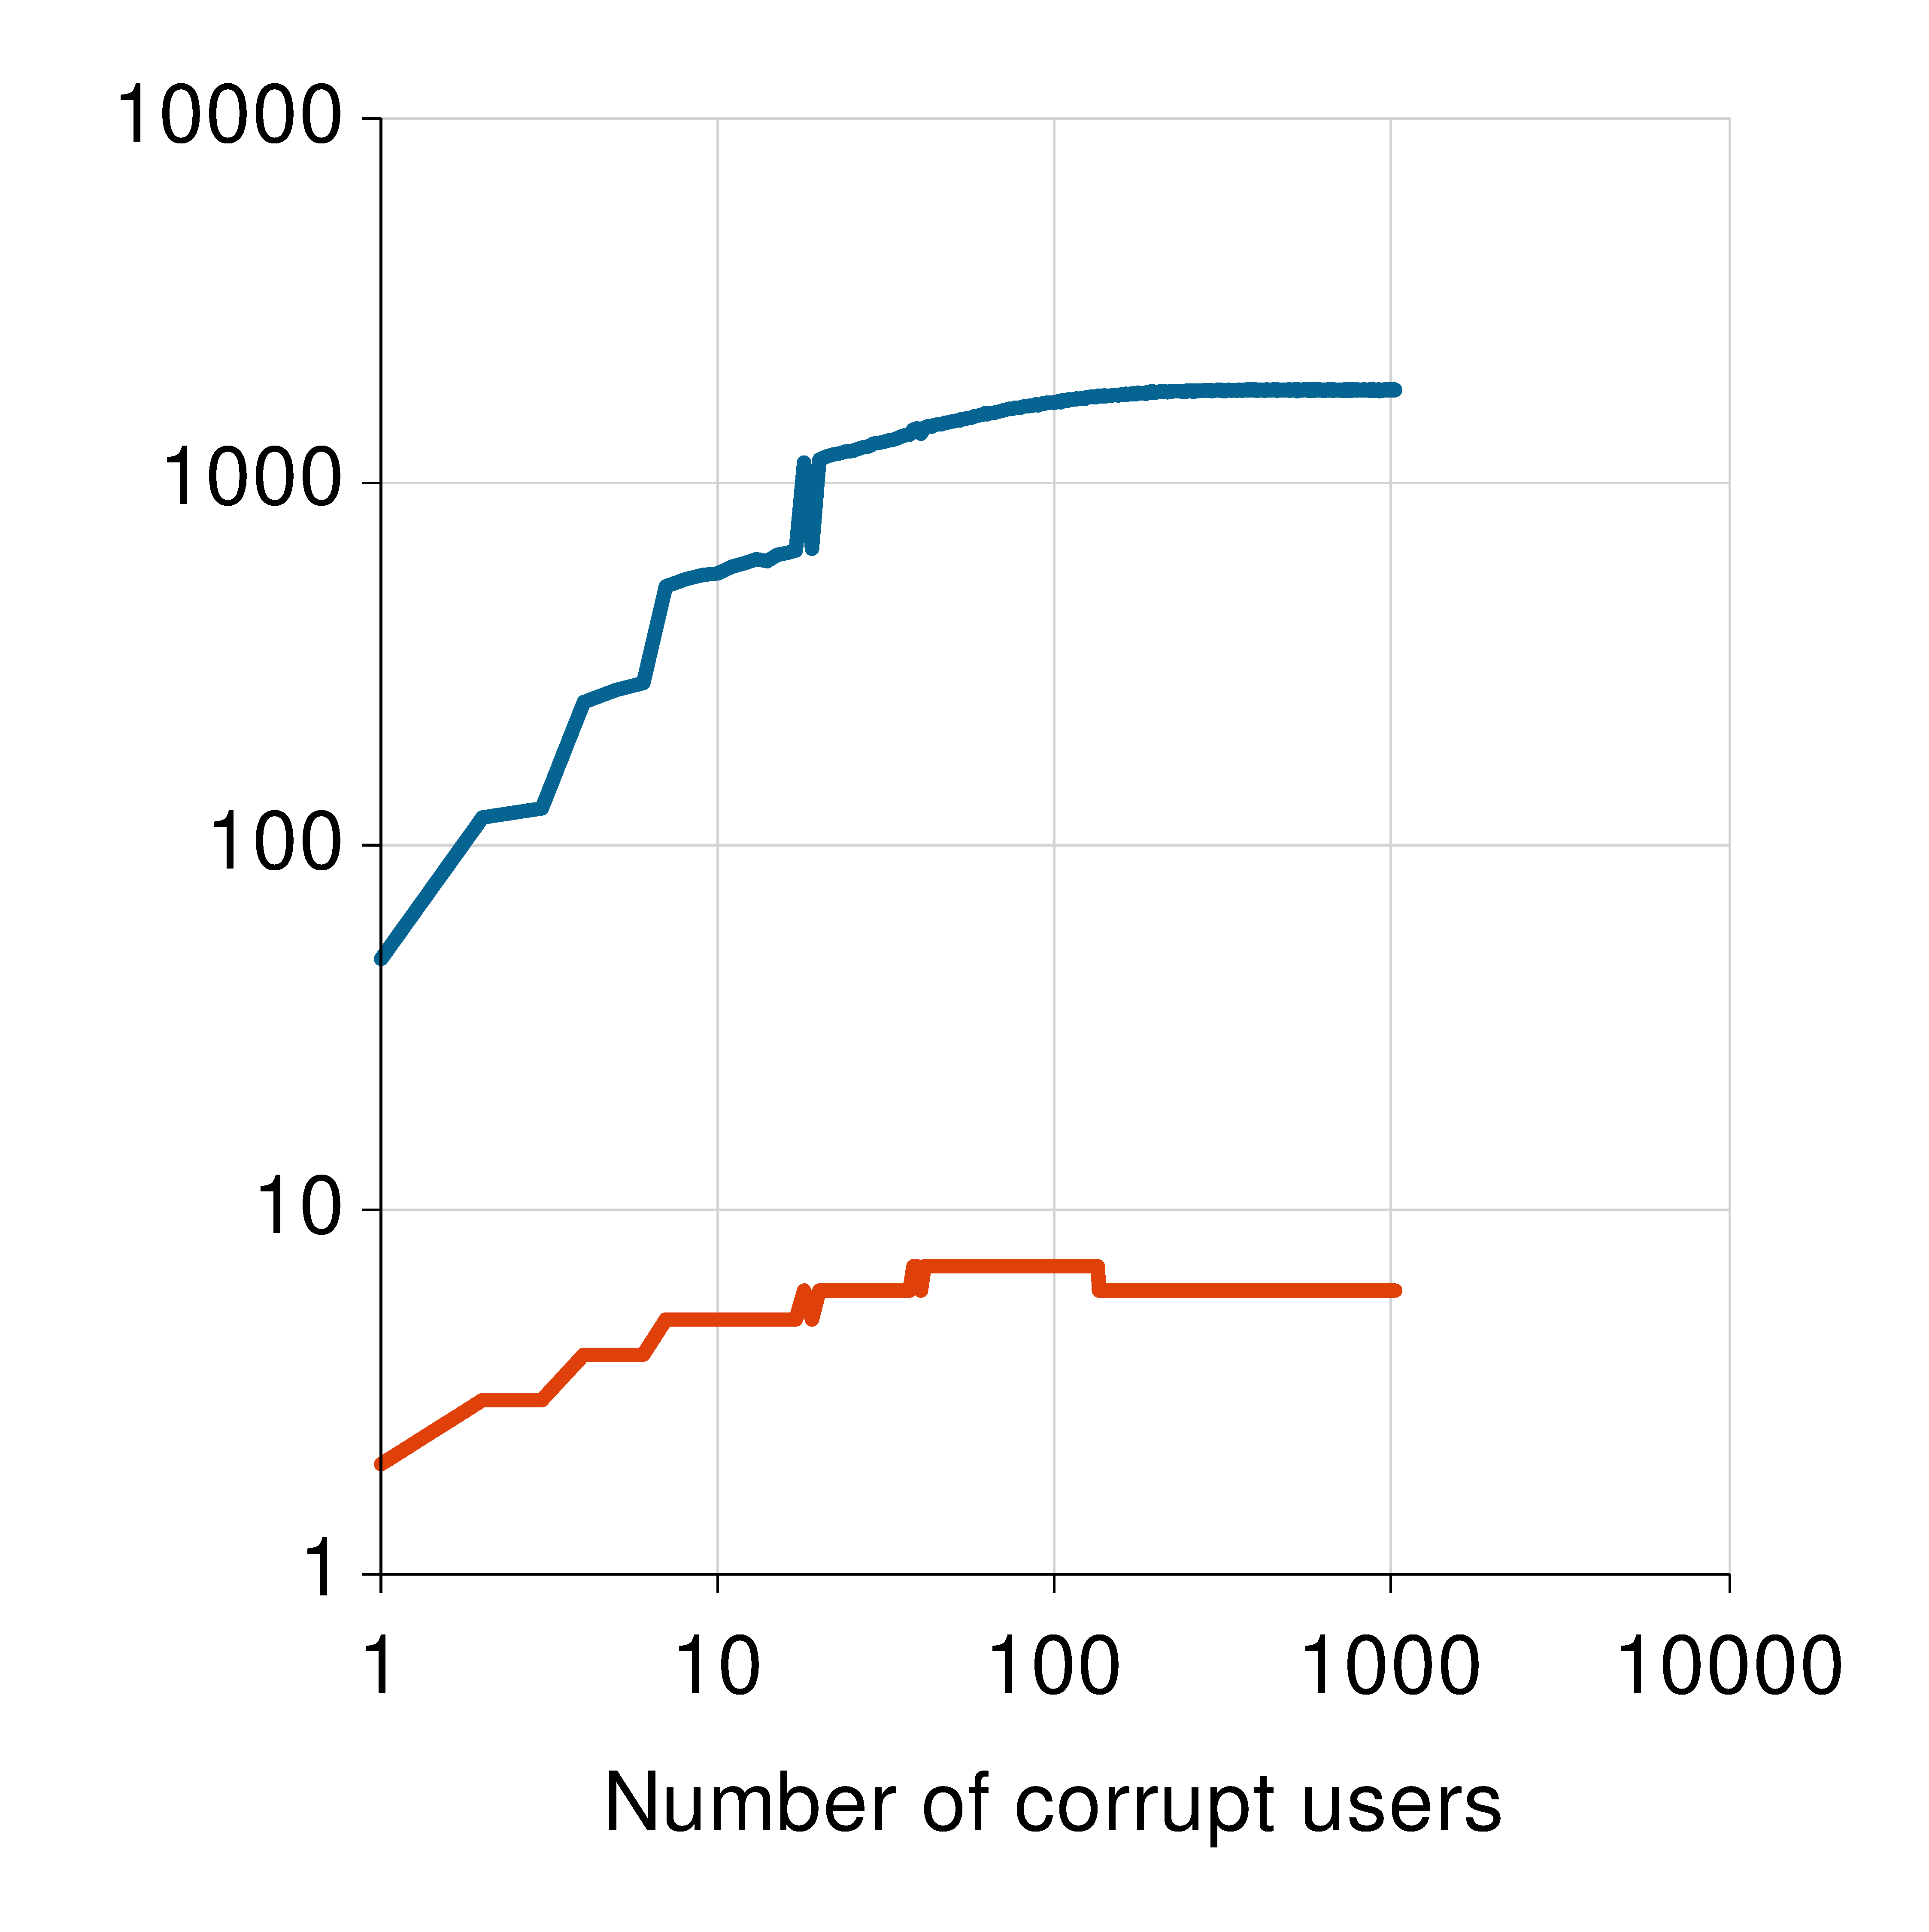
\includegraphics[width=0.35\textwidth]{images/plot-stochastic-VarT-1024}\caption{Simulation results for $n=1024$ and various number of corrupt users
		with aggressive (left) prudent (middle), and stochastic (right) adversary.}
	\label{fig:circuit-1-1} 
\end{figure*}

\section{Conclusion} \label{sec:conclusion}
We described bridge distribution algorithms that allow all (honest) users to connect to Tor in the presence of an adversary corrupting an unknown number of users. Our algorithms can adaptively increase the number of bridges according to the behavior of the adversary and use near-optimal number bridges.